\chapter{Backgrounds}\label{chapter:backgrounds}

\section{Estimation of backgrounds}\label{sec:background_estimation}

In the search for astrophysical neutrinos, the predominant backgrounds are from atmospheric neutrinos and atmospheric muons.
Single atmospheric neutrinos are able to produce the same event signatures as astrophysical neutrinos because they are not fundamentally different astrophysical neutrinos.
Atmospheric neutrinos can only be distinguished from their astrophysical counterparts by examining the population properties, or by the fact that muons produced in the same air shower can also reach the detector simultaneously.
Muons from cosmic ray air showers differ from neutrinos in their event signature as they always produce light while entering the detector, while neutrinos can interact within the detector volume before any light is produced near the edge of the detector.
Muons can also only be observed up to a certain amount of overburden, beyond which they will lose their energy and decay before reaching the detector.
This means the up-going observation region is free from atmospheric muons.

\subsection{Neutrino background estimation}

Atmospheric neutrinos are predominantly produced by the decay of pions and kaons, which we shall call the ``conventional'' component.
At energies above $\SI{1}\TeV$ the spectrum of the conventional component is softer than the incident cosmic-ray spectrum by one unit in the spectral index, due to the interactions of these mesons in the atmosphere.
The conventional neutrino flux is largest at the horizon, $\cos\theta_z=0$~\cite{Gaisser:2002jj,Barr:2004br,Honda:2006qj,Petrova:2012qf} because the larger path length in the thin atmosphere increases the proportion of pions that can decay before interacting.
To model the conventional neutrino flux, we use a parameterization of the Honda {\it{}et al.} 2006 flux calculation~\cite{Honda:2006qj} given in~\cite{Montaruli:2011as} which at the highest energies uses the analytic parameterization of the neutrino flux in~\cite{Gaisser:2002jj}.
This calculation is tuned to match observations of atmospheric muons, which remain difficult to predict from first principles.

A sub-leading -- yet unobserved -- contribution due to charmed hadron decays is expected to be important above $\sim\SI{100}\TeV$~\cite{Bhattacharya:2015jpa}.
Since the charmed hadrons decay promptly and do not interact in the atmosphere at the energies relevant for this analysis, we call this the ``prompt'' component.
Thus, at these energies, the prompt component has a spectral index close to the incident cosmic-ray spectrum.
The prompt flux is also constant with respect to the cosine of the zenith angle, as the short decay time of the charmed hadrons removes the effect of different path lengths through the atmosphere.
To model the prompt neutrino flux at Earth's surface, we use the flux computed in~\cite{Bhattacharya:2015jpa}.

The angular and energy distribution of the initial atmospheric neutrino flux is modified with respect to the flux at Earth's surface because of absorption of high-energy neutrinos in the Earth.
We account for this using a dedicated Monte Carlo, similar to the one described in~\cite{Gazizov:2004va}, that simulates the propagation of neutrinos in the Earth.
In this Monte Carlo we use the isoscalar neutrino cross sections given in~\cite{CooperSarkar:2011pa} for the neutrino-nucleon interactions, and the Earth density model described in~\cite{Dziewonski:1981xy}.
Neutrino-electron scattering can be safely neglected except for resonant-W production~\cite{Glashow:1960zz} which we include.
We ignore the uncertainties on the Earth opacity as they are known to be sub-leading in this energy range~\cite{Gandhi:1995tf,CooperSarkar:2011pa,Vincent:2017svp}.

Modeling the atmospheric neutrino flux with these two components does not account for the contribution of $K_s$~\cite{Gaisser:2014pda}, which is $\sim \SI{10}\percent$ at $\SI{100}\TeV$ and well-within our uncertainties.
In order to account for uncertainties in the cosmic-ray flux~\cite{Dembinski:2017zsh} and hadronic interactions~\cite{Fedynitch:2012fs} we parameterize the atmospheric neutrino flux as
\noindent
\begin{linenomath*}
	\begin{equation}
	\begin{split}
	\phi_\nu^{\rm{atm}} =& \Phi_{conv} \bigg(\phi^\pi_\nu + R_{K/\pi} \phi^K_\nu\bigg) {\bigg(\frac{E_\nu}{E_0^c} \bigg)}^{-\Delta \gamma_{CR}} \\ &+ \Phi_{prompt} \phi^p_\nu {\bigg(\frac{E_\nu}{E_0^p} \bigg)}^{-\Delta \gamma_{CR}},
	\end{split}
	\label{eq:atm_flux_equation}
	\end{equation}
\end{linenomath*}
where $\phi^\pi_\nu$, $\phi^K_\nu$, and $\phi^p_\nu$ are the conventional pion, kaon, and prompt atmospheric neutrino fluxes at a neutrino energy $E_\nu$ respectively.

The parameters $\convnorm$ and $\promptnorm$ are normalizations for the conventional and prompt normalizations respectively; $\pik$ allows us to modify the relative kaon to pion contributions; and the $\crdeltagamma$ parameter allows for hardening or softening of the atmospheric neutrino component to account for uncertainties in the cosmic-ray flux slope.
These parameters are incorporated into the analysis as nuisance parameters with priors as summarized in \reftab{tbl:priors}.
This analysis refrains from directly using prior information from other IceCube neutrino studies in order to provide results independent from other neutrino samples.

The conventional normalization prior is motivated by studies of the total uncertainty due to cosmic-ray and high-energy hadronic processes~\cite{Fedynitch:2012fs}; it is chosen to be Gaussian for simplicity with an expectation centered on the baseline flux model and appropriate variance.
The standard deviation of the Gaussian prior on the cosmic-ray slope parameter has been chosen to be $0.05$ in order to accommodate values measured at intermediate~\cite{Karelin:2011zz} and high~\cite{Bartoli:2015fhw,Yoon:2017qjx,Alfaro:2017cwx} energies.
The uncertainty on corrections to the ratios of neutrinos-to-anti-neutrinos ($\atmonunubar$) and kaon-pion yields ($\pik$) were estimated by comparing the expectation of different atmospheric neutrino calculations and a Gaussian prior width was chosen that encompasses their predictions.
Details regarding these corrections and the different atmospheric neutrino flux calculations can be found in~\cite{CollinFluxes,Jones:2015bya}.
Finally, the parameters $E_0^c=\SI{2020}\GeV$ and $E_0^p=\SI{7887}\GeV$ are points of fixed differential flux for the conventional and prompt components.

This simple parameterzation of the atmospheric neutrino flux and its uncertainties is chosen because it models the primary systematic effects of physical uncertainties that are observable with this sample.
Of course this neglects other physical uncertainties, such as those regarding the hadronic interactions in cosmic ray air showers and the composition of the cosmic ray particles.
But, these effects do not produce modifications to the observations that can be statistically discerned with the amount of data available.
Later it will be shown that even the modeled systematic uncertainties have a small effect on astrophysical measurements compared to the statistical uncertainties.

The above description models the flux of atmospheric neutrinos, but does not fully encapsulate the detector response to atmospheric neutrinos.
We have so far neglected the effect of accompanying muons on the detector response.
This is discussed at length in the next section.

% Table of all systematics and their priors if applicable
\begin{table*}[thb]
	\centering
	% systematic parameter & prior type & mean & sigma & min & max
	\begin{tabular}{l rrr}
		%\toprule
		%& \multicolumn{5}{c}{Prior information} \\
		%\cmidrule{2-6}
		Parameter & Prior (constraint) & Range & Description \\
		\toprule
		\multicolumn{1}{l }{\textbf{Astrophysical neutrino flux:}} & & & \\
		$\astronorm$ & - & $[0,\infty)$ & Normalization scale\\
		$\astrodeltagamma$ & - &  $(-\infty,\infty)$ & Spectral index\\
		%$\theta_a$ & Uniform &  &  & 0 & 1 \\ \hline
		%$\theta_b$ & Uniform &  &  & -1 & 1 \\ \hline
		%${2\nu/\left(\nu+\bar{\nu}\right)}_\texttt{astro}$ & - & $[0,2]$\\
		&&\\
		\midrule
		\multicolumn{1}{l }{\textbf{Atmospheric neutrino flux:}} & & &\\
		$\convnorm$ & $1.0\pm0.4$ & $[0, \infty)$ & Conventional normalization scale\\
		$\promptnorm$ & - & $[0, \infty)$ & Prompt normalization scale\\
		$\pik$ & $1.0\pm0.1$ & $[0, \infty)$ & Kaon-Pion ratio correction\\
		$\atmonunubar$ & $1.0\pm0.1$ & $[0,2]$ & Neutrino-anti-neutrino ratio correction\\
		&&\\
		\midrule
		\multicolumn{1}{l }{\textbf{Cosmic ray flux:}} & & &\\
		$\crdeltagamma$ & $0.0\pm 0.05$ & $(-\infty,\infty)$ & Cosmic-ray spectral index modification\\
		$\muonnorm$ & $1.0\pm 0.5$ & $[0,\infty)$ & Muon normalization scale\\
		&&\\
		\midrule
		\multicolumn{1}{l }{\textbf{Detector:}} & & &\\
		$\domeff$ & $0.99 \pm 0.1$ & $[0.80, 1.25]$ & Absolute energy scale\\
		$\holeice$ & $0.0 \pm 0.5$ & $[-3.82, 2.18]$ & DOM angular response\\
		$\anisotropy$ & $1.0 \pm 0.2$ & $[0.0, 2.0]$ & Ice anisotropy scale\\
	\end{tabular}
	\internallinenumbers
	\caption{\textbf{\textit{Analysis model parameters for the single power-law astrophysical model.}} Prior probabilities (constraints) for analysis parameters used in Bayesian (frequentist) analyses respectively.
		Priors (constraints) on the parameter are either uniform or Gaussian.
		Where applicable, the mean, standard deviation, and bounds are given.}\label{tbl:priors}
\end{table*}


\subsection{Atmospheric neutrino passing fractions}
\label{sec:passingfractions}
This discussion and study of atmospheric passing fractions is directly adapted from a collaborative work with Carlos A. Argüelles, Sergio Palomares-Ruiz, Logan Wille, and Tianlu Yuan~\cite{Arguelles:2018awr}.
Figures and equations are reproduced from~\cite{Arguelles:2018awr}, and the text follows the same thread of discussion.

As noted in~\cite{Schonert:2008is}, muons produced in the same air-shower may trigger the detector veto in coincidence with the neutrino interaction.
Dedicated simulations of cosmic ray air showers where neutrino interactions are forced can provide observational predictions for the distribution of these combined muon+neutrino events.
However, available simulation techniques to create these estimates remain prohibitively expensive for the desired accuracy.
Instead, we look to model this effect by computing an average efficiency with respect to the case where no muons reach the detector.
To account for this when weighting the neutrino-only simulation each atmospheric neutrino flux component, $i$, is multiplied by an efficiency.
This efficiency is referred to as the ``atmospheric neutrino passing fraction'', and denoted by $\mathcal{P}^{i,\alpha}_{passing}$, for each neutrino flavor $\alpha$.

The passing fraction depends on the details of air shower development, which includes modeling of the hadronic interaction, and the energy losses of muons in the material between the shower and the detector. 
Air-shower properties are averaged over in this calculation, but the passing fraction is still a probability that is conditional on the neutrino properties.
Of particular interest are the potential systematic dependencies of the passing fraction, which include the cosmic ray spectrum and composition, the hadronic interaction model, muon energy losses, and the atmospheric density model.
The calculation of the passing fraction is designed so that these systematic dependencies may be changed between different alternatives.
Additionally, the detector response enters in only one place in the formalism as a probability of muon rejection.
This allows for simple variation of the detector response modeling in a generic way.
To perform this calculation a framework was developed that leverages the Matrix Cascade Equation (MCEq) package in key portions of the calculation.
Validation of the computed passing fractions is performed against detailed air shower simulations with COsmic Ray SImulations for KAscade (CORSIKA), and excellent agreement is found as a result.

Departure from the lone-neutrino case is based on the coincidence of a muon and neutrino from the same air-shower that occurs in both time and direction.
Thus, $\Prob_{\rm reach}\left(\Emf \, | \, \Emi , \, X_\mu, \right)$ is naturally a key component of the calculation, which describes the probability of a muon with initial energy $\Emi$ and slant depth $X_\mu$ to reach the detector with energy $\Emf$.
As the IceCube detector is deep underground, the contribution to slant depth from the atmosphere is very small compared to that of the Earth, and so can be neglected.
With only the slant depth of the Earth contributing, $X_\mu$ is fully specified by the zenith angle $\theta_z$ in detector coordinates and the depth $d$.
Stochasticity of the muon energy losses is accounted for by the distribution $\Prob_{\rm reach}$, which is computed by tabulating simulations of muons propagated in ice by the software $\MMC$.
Using the conditional probability distribution $\Prob_{\rm reach}$ instead of average muon behavior ensures that contributions from the distribution tails are accounted for.
These contributions from the tails become important for very large slant depths, where muons on average do not reach the detector.
Departure from the neutrino-only case requires both the muon to reach the detector, but also for the muon to trigger a response, in this case for the muon to {\it light} the veto.
The quantity $\Prob_{\rm light}(\Emf,d)$ is the probability that a muon of energy $\Emf$ and depth $d$ at the detector boundary {\it lights} the veto, such that the event is rejected.
In practice, this $\Prob_{\rm light}$ is computed by tabulating detector simulations of atmospheric muons and incorporating the specifics of the event selection.
With both $\Prob_{\rm light}$ and $\Prob_{\rm reach}$ in hand, the probability of detecting an incident muon $\Prob_{\rm det}$ can be computed as 

\begin{equation}
\label{eq:PrPl}
\Prob_{\rm det}\left(\Emi , \, X_\mu(\theta_z, d), d\right) \equiv \int d\Emf \, \Prob_{\rm reach}\left(\Emf \, | \, \Emi , \, X_\mu(\theta_z, d)\right) \, \Prob_{\rm light} (\Emf, d) ~.
\end{equation}

Note that losses also depend on the medium and not only on the slant depth, whose dependence on $\theta_z$ we write explicitly. If the medium surrounding the detector is homogeneous, the dependence on $X_\mu$ can be exchanged for distance without loss of generality.
From here on to simplify the notation, the dependence on $X_\mu$ will be replaced by a dependence on $\theta_z$ and the dependence on $d$ will be neglected.
These dependencies can be added back in at the end of the calculation without any change to the result.

\begin{figure}
	\centering
    \begin{subfigure}{\linewidth}
		\centering
		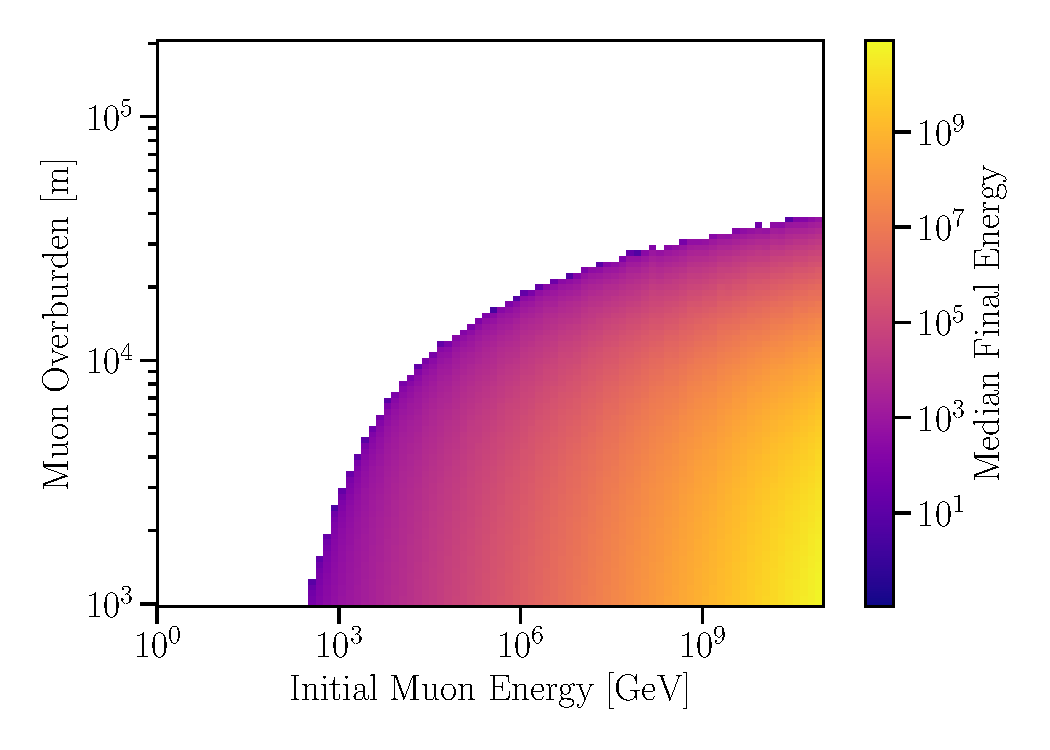
\includegraphics[width=0.8\linewidth]{figures/preach_median}
	\end{subfigure}
	\begin{subfigure}{\linewidth}
		\centering
		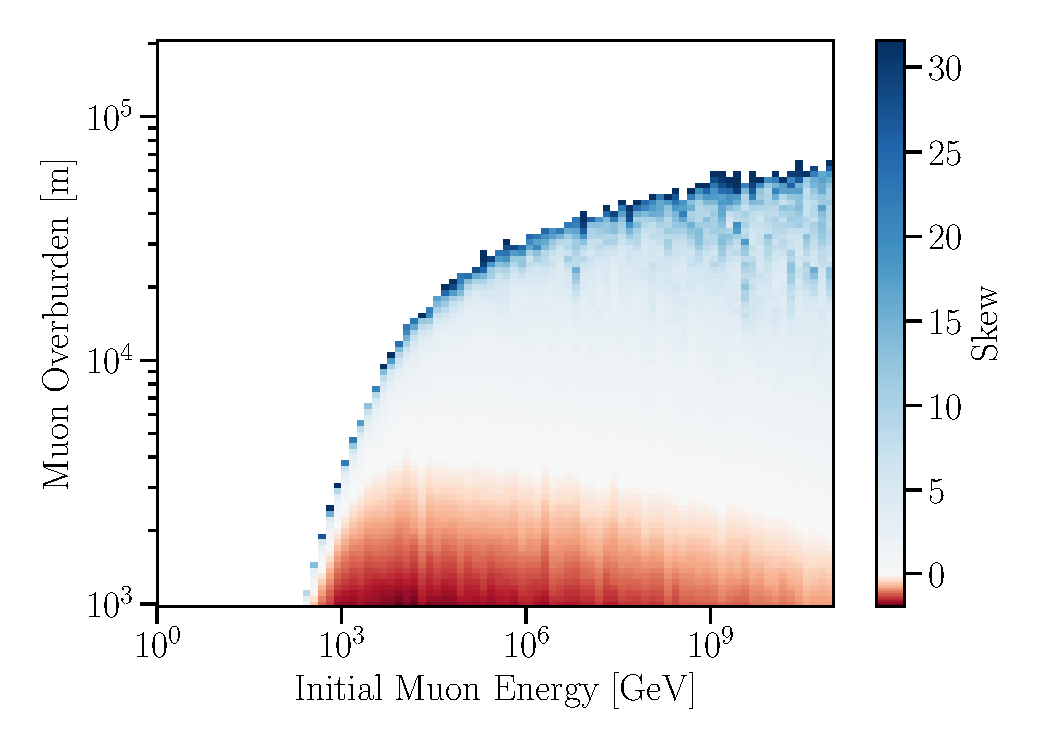
\includegraphics[width=0.8\linewidth]{figures/preach_skew}
	\end{subfigure}
	\caption{\textbf{\textit{Muon Final Energy Statistics.}} Muons propagating in ice were simulated for a wide range of initial energies, and at a set of predefined distances their energy was recorded.
	This results in a distribution of final muon energies for each combination of initial muon energy and overburden.
	These two plots show statistics of these distributions, with the upper plot displaying the median and the lower plot displaying the skew.
	Previous calculations only used the median of these distributions.
	However, the large skew of these distributions shows us that the tails become important for large overburdens.
	}
	\label{fig:preach_stats}
\end{figure}

The atmospheric neutrino passing fraction is defined as the probability for an atmospheric neutrino to not be accompanied by a muon which is detected from the same air shower. This probability is denoted $\Prob_{\rm pass}$~\cite{Schonert:2008is, Gaisser:2014bja} and can be written as the ratio
\begin{equation}
\Prob_{\rm pass} (E_\nu, \theta_z) = \frac{\phi_\nu^{\rm pass}(E_\nu, \theta_z)}{\phi_\nu(E_\nu, \theta_z)} ~,
\end{equation}
where $E_\nu$ is the neutrino energy, $\theta_z$ is the zenith angle, $\phi_\nu^{\rm pass}$ is the differential flux of atmospheric neutrinos accompanied by muons that are detected, and $\phi_\nu$ is the total differential atmospheric neutrino flux.
In the next sections, passing fractions for electron neutrinos and muon neutrinos are derived.
As tau neutrinos by comparison make up a very small portion of the atmospheric flux, there is no dedicated discussion for this case.
However, the concerns for tau neutrinos are very similar to those of electron neutrinos minus the differences in their production.

\subsubsection{$\nu_e$ passing fraction}
Electron neutrinos (or antineutrinos) are produced alongside a positron (or electron) in the decay of their parent particle, for example $K^+ \rightarrow \pi^0 + e^+ + \nu_e$.
Rarely does an electron neutrino have a sibling muon, as this would involve a lepton flavor violating process.
Instead, muons that accompany electron neutrinos are produced in other branches of the air shower.
Because the different branches of the shower are uncorrelated, to first order the average properties of muons in a prototypical air shower can be used for the passing fraction calculation.
Consider a shower from a single cosmic-ray primary particle of type $A$ with energy $\ECR$.
The average neutrino yield $\frac{dN_{A, \nu}}{dE_\nu}(\ECR, E_\nu, \theta_z)$ from such a shower can be computed with $\MCEq$.
So the atmospheric neutrino flux can be written as 
\begin{equation}
\label{eq:nuphi}
\phi_\nu(E_\nu, \theta_z)  = \sum_A \int d\ECR \, \frac{dN_{A, \nu}}{dE_\nu}(\ECR, E_\nu, \theta_z) \, \phi_A(\ECR)~,
\end{equation}
where $\phi_A(\ECR)$ is the flux of primary cosmic rays of type A.
the passing fraction can be obtained by modifying the integrand of Eq.~\ref{eq:nuphi} so that it is weighted by the Poisson probability $Pzmproto$ of detecting an accompanying muon.
In this way the uncorrelated passing fraction can be written as
\begin{equation}
\label{eq:PuncorGJKvS}
\Prob_{\rm pass}^{\rm uncor, GJKvS}(E_\nu, \theta_z)  =  \frac{1}{\phi_\nu(E_\nu, \theta_z)} \sum_A \int d\ECR \, \frac{dN_{A, \nu}}{dE_\nu}(\ECR, E_\nu, \theta_z) \, \phi_A(\ECR) \, \Pzmproto \left(N_\mu = 0  ; \bar N_{A, \mu}^{\rm GJKvS}(\ECR, \theta_z)\right)~,
\end{equation}
where $\Pzmproto \left(N_\mu = 0  ; \bar N_{A, \mu}^{\rm GJKvS}(\ECR, \theta_z)\right) = \exp{-\bar N_{A, \mu}^{\rm GJKvS}(\ECR, \theta_z)}$,
and  $\bar N_{A, \mu}^{\rm GJKvS}(\ECR, \theta_z)$ is the average number of muons that are detected from an air shower.
This average number of muons is computed using the yield of muons from the air shower $dN_{A, \mu}/d\Emi(\ECR, \Emi)$ and the probability of detecting those muons, such that
\begin{equation}
\label{eq:Nmu}
\bar N_{A, \mu}^{\rm GJKvS}(\ECR,\theta_z) = \int d\Emi \, \frac{dN_{A, \mu}}{d\Emi}(\ECR, \Emi,  \theta_z) \, \Prob_{\rm det}\left(\Emi , \theta_z\right) ~,
\end{equation}
Some terms in the above equations are labeled with ${\rm GJKvS}$ because these quantities are calculated in the same manner as was done in~\cite{Gaisser:2014bja} under certain choices for $\Prob_{\rm det}$.
Namely, when $\Prob_{\rm light}$ is defined as a Heaviside function with a boundary at $\Emf = \SI{1}\TeV$, and $\Prob_{\rm reach}$ is defined as a delta function that matches the initial muon energy to the median final muon energy.

Fig.~\ref{fig:nue_passing-preach-effect} shows the effect of the two muon treatments on the passing fractions as defined in Eq.~\ref{eq:PuncorGUE}.
At the horizon the median approximation overestimates the passing fraction while near the vertical direction it is underestimated.
In the horizontal region, muons with smaller initial energy such that their median range is less than the distance to the detector represent a small but non-negligible fraction of muons that may trigger the detector veto.
Thus, in the median muon treatment the passing fraction is overestimated because of too few muons.
In the vertical region, with less overburden the probability for muon detection rapidly increases to approximately one with initial muon energy, however this turnover is faster with the median treatment than the full treatment.
This means more muons contribute to the calculation in the median case and the passing fraction is underestimated.

\begin{figure}
	\centering
	\subfloat{
		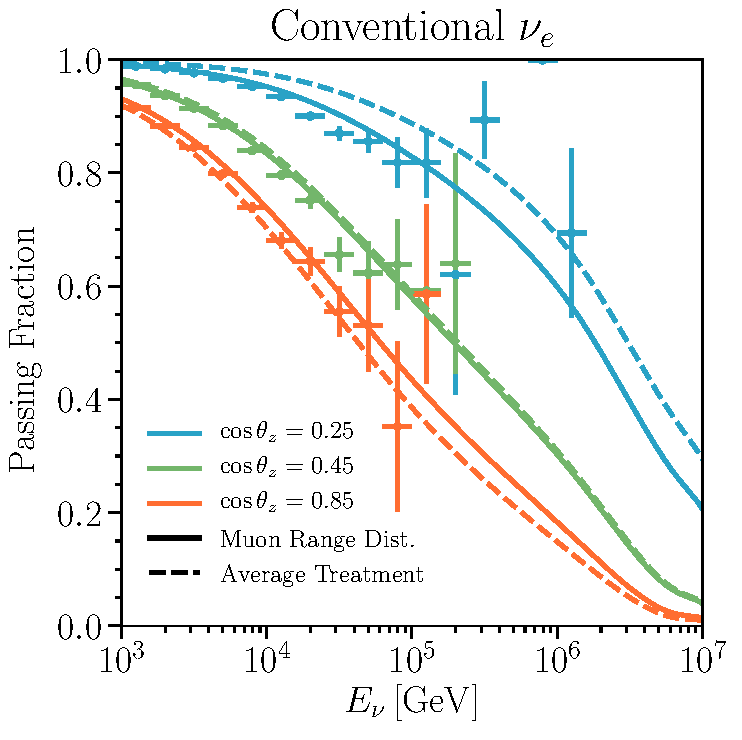
\includegraphics[width=0.45\linewidth]{results/passing_fractions_paper/fig/fig4_nue_conv_murange_vs_avg}
	}
	\subfloat{
		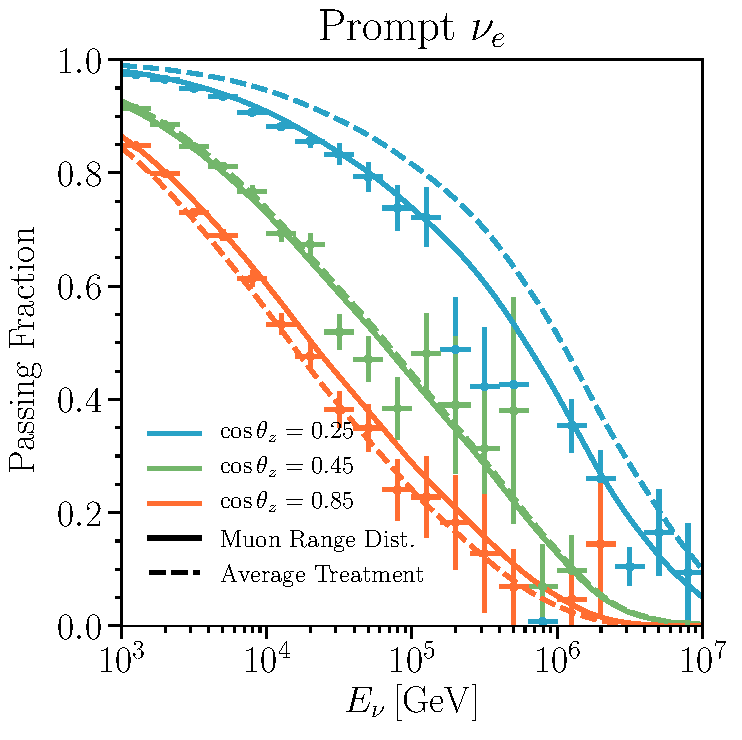
\includegraphics[width=0.45\linewidth]{results/passing_fractions_paper/fig/fig4_nue_prompt_murange_vs_avg}
	}    
	\caption{\textbf{\textit{Passing fractions: effect of the treatment of muon losses in ice.}} Results are shown for three values of $\cos\theta_z$ (from top to bottom): 0.25 (blue), 0.45 (green), and 0.85 (orange); using the full muon range distribution (solid) or the median muon range (dashed). Results from the \CORSIKA{} simulation are shown as crosses, with statistical error bars only. In all cases, the H3a primary cosmic-ray spectrum~\cite{Gaisser:2011cc}, the SIBYLL~2.3 hadronic-interaction model~\cite{Engel:2015dxa, Riehn:2015oba} and the MSIS-90-E atmosphere-density model at the South Pole on July 1, 1997~\cite{Labitzke:1985, Hedin:1991} are used. A depth in ice of $d_{\rm det} = \SI{1.95}\km$ (like the center of IceCube) and a Heaviside $\Prob_{\rm light}(\Emf) = \Theta(\Emf - 1\,{\rm TeV})$ are assumed. \textit{Left panel:} Conventional $\nu_e$ passing fraction. \textit{Right panel:} Prompt $\nu_e$ passing fraction.
	}
	\label{fig:nue_passing-preach-effect}
\end{figure}

In Eq.~\ref{eq:Nmu} the energy available to other branches of the shower to produce uncorrelated muons is over estimated as some energy must be reserved for producing the electron neutrino or rather the branch of the shower that produces the electron neutrino.
A complete modeling of the connection between the three relevant particles (cosmic ray primary, the electron neutrino, and muons) is cumbersome, as it would involve modeling the shower branch producing the electron neutrino in its entirety and then separately modeling the uncorrelated branch.
However, a simple approximation can be made that at least accounts for the energy necessary to produce the electron neutrino.
The electron neutrino must be produced by a parent particle $p$ that has a kinematically allowed energy $E_p$, so the remaining energy is $\ECR-E_p$.
The muon yield is then modeled using the average behavior of a shower that begins with energy $\ECR-E_p$.
Because we are now concerned with the parent particle of the electron neutrino, the slant depth through which this parent particle travels must be considered, as this will affect the probability that it decays to a neutrino instead of interacting.
Now considering the parent particle energy and slant depth, the yield of neutrinos from the air shower can be expanded as
\begin{equation}
\label{eq:Anuyield}
\frac{dN_{A, \nu}}{dE_\nu}(\ECR, E_\nu, \theta_z) = \int dE_p \, \int \frac{dX}{\lambda_p(E_p, X)} \, \frac{dN_{p, \nu}}{dE_\nu}(E_p, E_\nu) \, \frac{dN_{A, p}}{dE_p}(\ECR, E_p, X) ~,
\end{equation}
where $dN_{p, \nu}/dE_\nu(E_p,E_\nu)$ is the spectrum of neutrinos from a parent particle $p$ with energy $E_p$, $dN_{A, p}/dE_p(\ECR,E_p,X)$ is the spectrum of parent particles from the air shower at slant depth $X$, and $dX/{\lambda_p(E_p, X)}$ is the probability of the parent to decay between the slant depth $X$ and $X+dX$.
$\lambda_p(E_p, X)$ is the product of the local density and the parent decay length such that $\lambda_p(E_p, X)=\rho(X) \tau_p E_p/m_p$, where $\rho(X)$ is the local density, $\tau_p$ is the lifetime of the parent, $E_p$ is its energy, and $m_p$ is its mass.
Now Eq.~\ref{eq:PuncorGJKvS} can be rewritten with the above expansion and the simple approximation that accounts for the available energy,
\begin{align}
\label{eq:PuncorGUE}
\Ppuncor (E_\nu, \theta_z) & = \frac{1}{\phi_\nu(E_\nu, \theta_z)} \, \sum_A \sum_{p} \int dE_p \int \frac{dX}{\lambda_p(E_p, X)} \int d\ECR \nonumber \\
& \frac{dN_{p, \nu}}{dE_\nu}(E_p, E_\nu) \, \frac{dN_{A, p}}{dE_p}(\ECR, E_p, X) \, \phi_A(\ECR) \, \Pzmproto \left(N_\mu = 0  ; \bar N_{A, \mu}(\ECR - E_p, \theta_z)\right) ~.
\end{align}
This treatment remains consistent with the calculation of the neutrino flux mentioned earlier, as if the Poisson probability of muon non-detection is removed (i.e. $\Pzmproto=1$) then the passing fraction is $1$ by construction.

The na\"ive approximation of the muon yield using $\ECR$ without the subtraction of $E_p$ tends to underestimate the passing fraction as can bee seen in Fig.~\ref{fig:nue_passing-double-counting}.
This is because the muon yield is larger for showers of greater energy.
Below $\SI{100}\TeV$ the absolute difference between the two methods is below $0.05$, however at higher energies and especially more vertical directions the relative difference becomes more important.

\begin{figure}
	\centering
	\subfloat{
		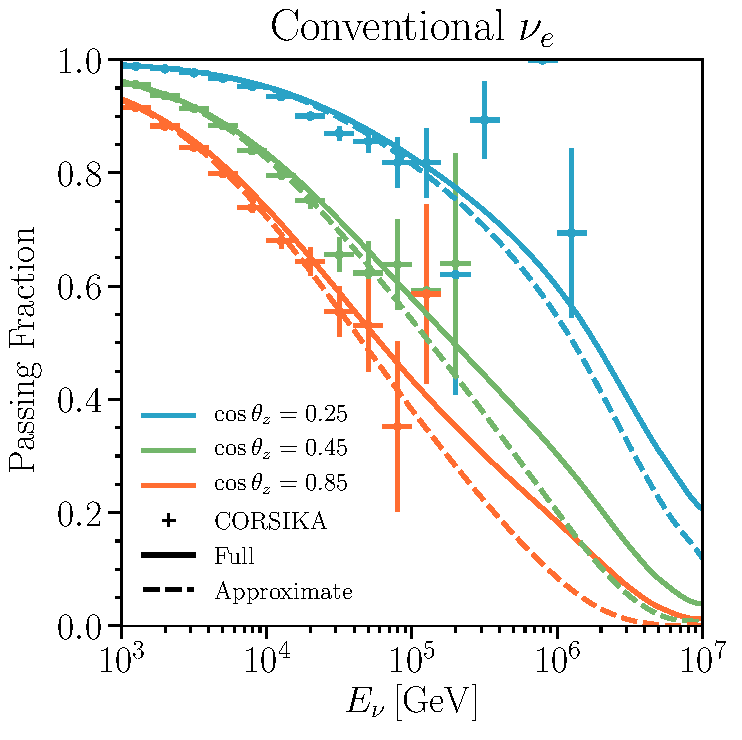
\includegraphics[width=0.45\linewidth]{results/passing_fractions_paper/fig/fig3_b_nue_conventional_unified_versus_factorized_with_corsika_sibyll_23}
	}
	\subfloat{
		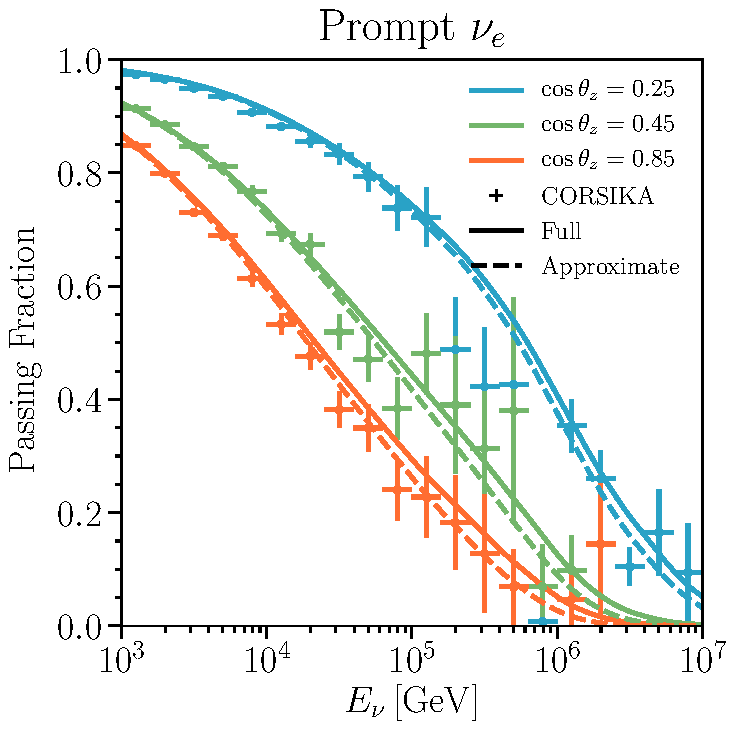
\includegraphics[width=0.45\linewidth]{results/passing_fractions_paper/fig/fig3_a_nue_prompt_unified_versus_factorized_with_corsika_sibyll_23}
	}
	\caption{\textbf{\textit{Passing fractions: effect of approximations on the energy of the shower giving rise to uncorrelated muons.}} Results are shown for three values of $\cos\theta_z$ (from top to bottom): 0.25 (blue), 0.45 (green), and 0.85 (orange); with the approach of this work (solid), Eq.~(\ref{eq:PuncorGUE}), where the energy carried by the neutrino parent is subtracted from the rest of the shower which produces the muons to be triggered (i.e., $\ECR - E_p$), and without this subtraction (dashed), Eq.~(\ref{eq:PuncorGJKvS}), considering the cumulative muon yield from a shower with energy $\ECR$. Results from the \CORSIKA{} simulation are shown as crosses, with statistical error bars only. \textit{Left panel:} Conventional $\nu_e$ passing fraction. \textit{Right panel:} Prompt $\nu_e$ passing fraction.
	}
	\label{fig:nue_passing-double-counting}
\end{figure}

Fig.~\ref{fig:nu-e-neutrino-vs-antineutrino} shows a comparison between this calculation and results from the CORSIKA simulation in addition to the differences between electron neutrino and antineutrino fluxes.
The agreement between simulation and this calculation modeling is excellent for
both neutrinos and antineutrinos.
The conventional electron antineutrino passing fractions are lower than those of conventional electron neutrinos, primarily because positively charged mesons are preferentially produced, leading to a harder spectrum than the negatively charged mesons.
The passing fractions for the prompt flux are almost identical as they are mainly produced from gluon fusion~\cite{Arguelles:2015wba}.

\begin{figure}
	\centering
	\subfloat{
		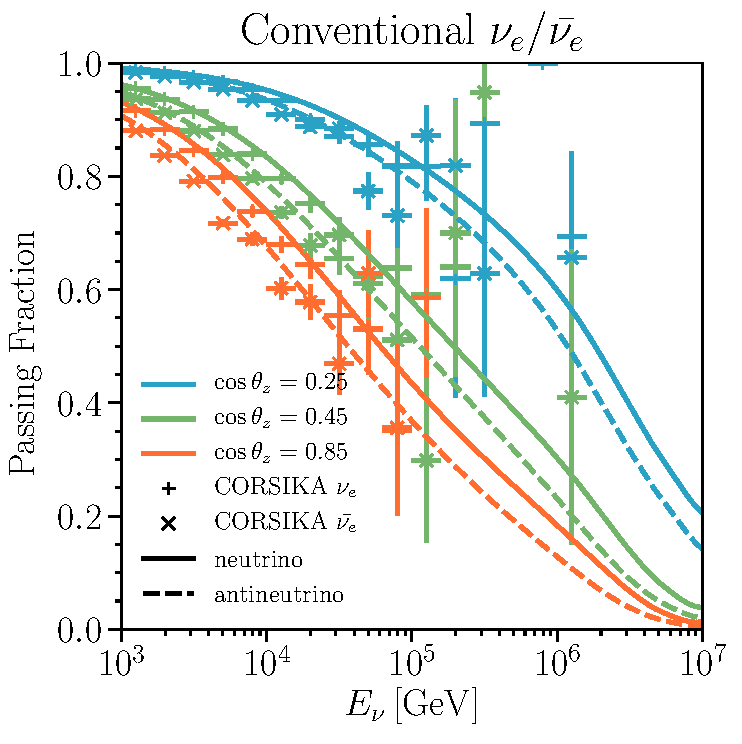
\includegraphics[width=0.45\linewidth]{results/passing_fractions_paper/fig/fig5_nue_conv_nu_vs_nubar}
	}
	\subfloat{
		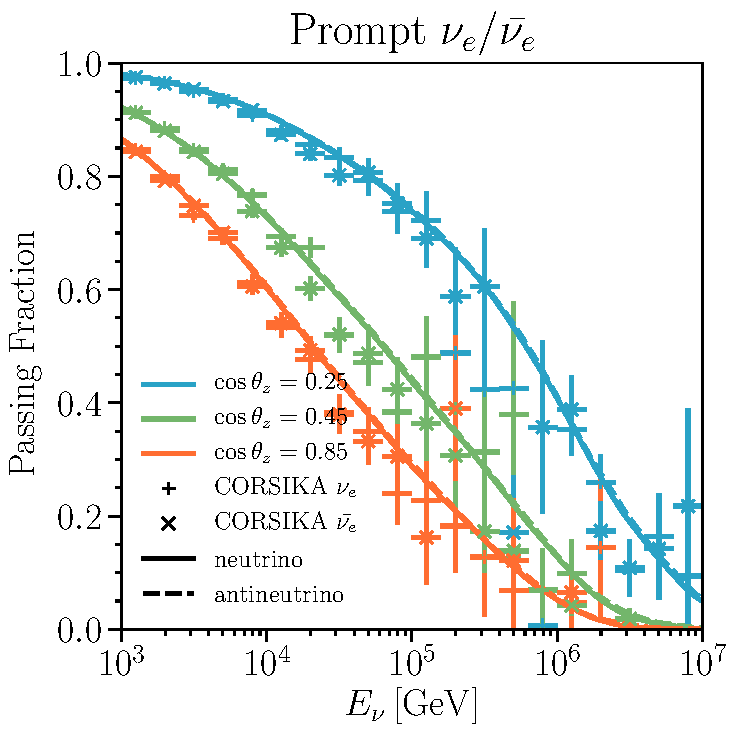
\includegraphics[width=0.45\linewidth]{results/passing_fractions_paper/fig/fig5_nue_prompt_nu_vs_nubar}
	}
	\caption{\textbf{\textit{Passing fractions: neutrinos versus antineutrinos.}} Results are shown for three values of $\cos\theta_z$ (from top to bottom): 0.25 (blue), 0.45 (green), and 0.85 (orange); for neutrinos (solid) and antineutrinos (dashed). Results from the \CORSIKA{} simulation for neutrinos ($+$) and antineutrinos ($\times$) are also shown, with statistical error bars only. In all cases, the H3a primary cosmic-ray spectrum~\cite{Gaisser:2011cc}, the SIBYLL~2.3 hadronic-interaction model~\cite{Engel:2015dxa, Riehn:2015oba} and the MSIS-90-E atmosphere-density model at the South Pole on July 1, 1997~\cite{Labitzke:1985, Hedin:1991} are used, and $d_{\rm det} = 1.95$~km in ice and $\Prob_{\rm light}(\Emf) = \Theta(\Emf - 1\,{\rm TeV})$ are assumed. \textit{Left panel:} Conventional $\nu_e$ passing fraction. \textit{Right panel:} Prompt $\nu_e$ passing fraction. Note that for prompts there are not differences between $\nu_e$ and $\bar\nu_e$.
	}
	\label{fig:nu-e-neutrino-vs-antineutrino}
\end{figure}

\subsubsection{$\nu_\mu$ passing fraction}

Muon neutrinos or antineutrinos produced in hadron decays will always have a sibling muon due to flavor conservation.
This means the passing fraction for muon neutrinos has a correlated component in addition to the uncorrelated component described for electron neutrinos.
This correlated suppression depends entirely on the behavior of the sibling muon, which itself can be described as a function of the muon direction and initial energy.
For two body decays, there is a direct relation between the energy of the parent particle, muon, and neutrino: $\Emi = E_p - E_\nu$.
This relation gives a delta function for the muon energy spectrum $dN_{p,\mu}^{\rm 2-body}/d\Emi (E_p,E_\mu,\Emi)=\delta(\Emi-E_p+E_\nu)$.
However, the two-body approximation is not appropriate for the calculation of the passing fractions for the prompt fluxes, as neutrinos are mainly produced by the decays of $D^{\pm}$, $D^0$, $\bar{D}^0$, $\Lambda_c^+$, and $D_s^{\pm}$~\cite{Fedynitch:2015zma}.
Treatment of $n$-body decays requires evaluating the muon distributions from the decays of these particles and using Eq.~(\ref{eq:pnomusib}).
In this work, $dN_{p, \mu}/d\Emi$ was generated for $K^0_L$, $D^+$, $D^0$, and $D^+_s$.\footnote{The decay distributions for their antiparticles are identical.}
For general $n$-body decays the probability of not detecting this sibling muon is a function of the energy spectrum and can be written as
\begin{equation}
\label{eq:pnomusib}
\Pzmsib \left(\theta_z|E_p, E_\nu \right) = 1 - \int d\Emi \, \Prob_{\rm det}\left(\Emi, \theta_z\right) \frac{dN_{p, \mu}}{d\Emi}(E_p, E_\nu, \Emi) ~.
%\Prob(\Emi|E_p, E_\nu) ~.
\end{equation}
Neglecting for a moment the uncorrelated muons, we can think about the correlated passing fraction as a separate calculation.
To obtain the correlated passing fraction we can start with the calculation of the neutrino flux, expanding to show the integration over the parent energy and slant depth as was done in Eq.~\ref{eq:Anuyield}.
\begin{equation}
\label{eq:nufluxcorexpanded}
\phi_\nu(E_\nu, \theta_z) = \sum_A \sum_{p} \int dE_p  \int \frac{dX}{\lambda_p(E_p, X)} \, \int d\ECR \, \frac{dN_{p, \nu}}{dE_\nu}(E_p, E_\nu) \, \frac{dN_{A, p}}{dE_p}(\ECR, E_p, X) \, \phi_{\rm A} (\ECR).
\end{equation}
To simplify notation, the flux of parent particles in the air shower at slant depth $X$ defined as
\begin{equation}
\label{eq:phip}
\phi_{A, p}(E_p, X) = \int d\ECR \, \frac{dN_{A, p}}{dE_p}(\ECR, E_p, X) \, \phi_{\rm A} (\ECR) ~,
\end{equation}
can be separated to obtain a more compact form for the neutrino flux
\begin{equation}
\label{eq:nufluxcor}
\phi_\nu(E_\nu, \theta_z) = \sum_A \sum_{p} \int dE_p  \int \frac{dX}{\lambda_p(E_p, X)} \, \frac{dN_{p, \nu}}{dE_\nu}(E_p, E_\nu) \, \phi_{A, p}(E_p, X).
\end{equation}
Again, weighting the integrand by the probability of detecting the muon, in this case the sibling muon, the correlated passing fraction can be written as
\begin{equation}
\label{eq:Pcor}
\Ppcor(E_\nu, \theta_z) = \frac{1}{\phi_\nu(E_\nu, \theta_z)} \, \sum_A \sum_{p} \int dE_p \int \frac{dX}{\lambda_p(E_p, X)} \, \frac{dN_{p, \nu}}{dE_\nu}(E_p, E_\nu) \, \phi_{A, p}(E_p, X) \, \Pzmsib \left(\theta_z|E_p, E_\nu \right).
\end{equation}

\begin{figure}
	\centering
	\subfloat{
		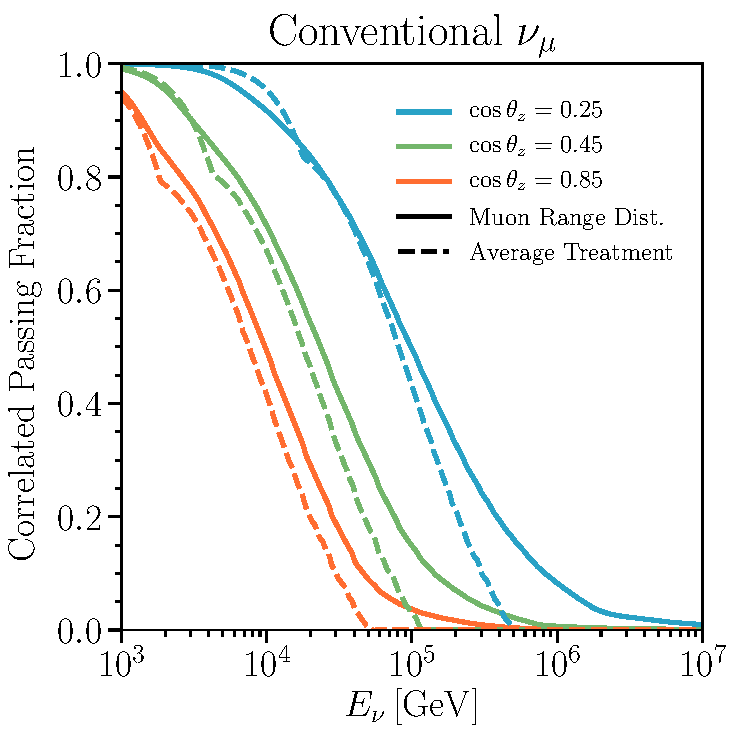
\includegraphics[width=0.45\linewidth]{results/passing_fractions_paper/fig/fig6_numu_conv_corr_only_murange_vs_avg}
	}
	\subfloat{
		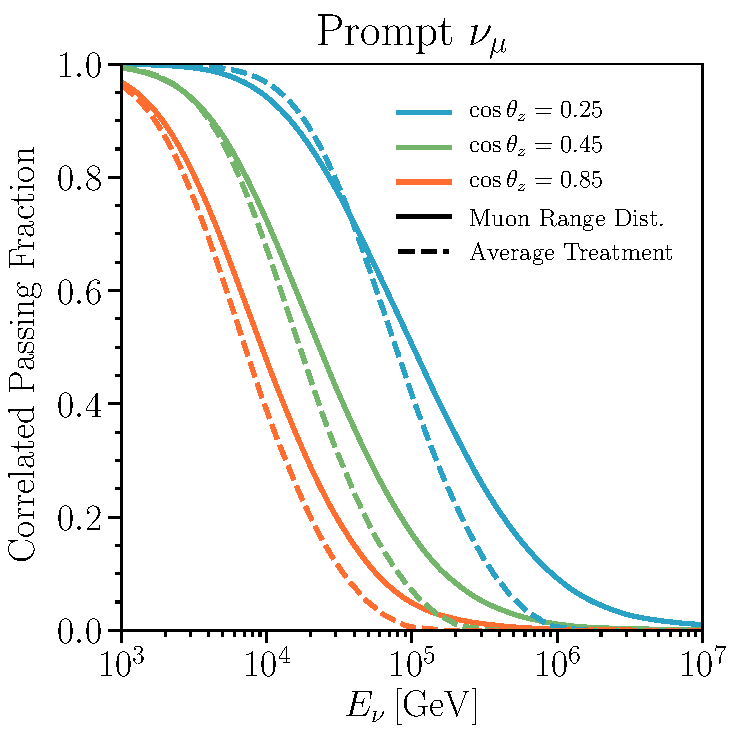
\includegraphics[width=0.45\linewidth]{results/passing_fractions_paper/fig/fig6_numu_prompt_corr_only_murange_vs_avg}
	}
	\caption{\textbf{\textit{Correlated passing fractions: effect of the treatment of muon losses in ice.}} Same as Fig.~\ref{fig:nue_passing-preach-effect} but only for the correlated part of the passing fraction for $\nu_\mu$.}
	\label{fig:nu-mu-correlated-preach-effect}
\end{figure}

In the same way that we compared different muon treatments for the uncorrelated passing fraction, Fig.~\ref{fig:nu-mu-correlated-preach-effect} shows the effect for the correlated passing fraction.
As the correlated case is only concerned with a single muon where energy is correlated with the neutrino, and energy dependent effect emerges.
For lower energies the muon detection probability is underestimated with the median treatment, resulting in a passing fraction that is too high while the converse is true for higher energies.
This effect is less pronounces in the horizontal region, as the energy correlation becomes more washed out with larger overburden.

As an approximation to the passing fraction, the correlated and uncorrelated passing fractions can be multiplied together like in~\cite{Gaisser:2014bja}.
Using the median muon behavior, the $2$-body approximation, and multiplying the two passing fractions we can obtain the same approximation to the passing fraction as in~\cite{Gaisser:2014bja}
\begin{equation}
\label{eq:PGJKvS}
\Prob_{\rm pass}^{\rm GJKvS} (E_\nu, \theta_z) \equiv \Prob_{\rm pass}^{\rm cor, SGRS}(E_\nu, \theta_z) \, \Prob_{\rm pass}^{\rm uncor, GJKvS}(E_\nu, \theta_z) ~,
\end{equation}
which contains the correlated passing fraction derived in~\cite{Schonert:2008is}
\begin{equation}
\label{eq:PcorSGRS}
\Prob_{\rm pass}^{\rm cor, SGRS}(E_\nu, \theta_z) = \frac{1}{\phi_\nu(E_\nu, \theta_z)} \, \sum_A \sum_{p} \int dE_p  \int \frac{dX}{\lambda_p(E_p, X)} \, \frac{dN_{p, \nu}}{dE_\nu}(E_p, E_\nu) \, \phi_{A, p}(E_p, X) \,
\left[1 - \Prob_{\rm det}^{\rm SGRS}\left(E_p-E_\nu , \theta_z\right)\right]~.
\end{equation}

Instead of taking the ``factorized'' approach in Eq.~\ref{eq:PGJKvS}, the correlated and uncorrelated equations can be combined at the level of muon detection, as the veto can be thought of as a logical OR between the detection of an uncorrelated muon and the detection of a sibling muon.
This logical OR can be achieved in the calculation by the multiplication of the non-detection probabilities $\Pzm = \Pzmsib \Pzmproto$.
Similarly weighting the integrand in the neutrino flux calculation by this quantity and maintaining the energy correction described previously, the complete passing fraction is obtained
\begin{align}
\label{eq:GUE}
\Prob_{\rm pass}(E_\nu, \theta_z) = \frac{1}{\phi_\nu(E_\nu, \theta_z)} \, \sum_A \sum_{p} & \int dE_p  \int \frac{dX}{\lambda_p(E_p, X)} \int d\ECR \, \frac{dN_{p, \nu}}{dE_\nu}(E_p, E_\nu) \, \frac{dN_{A, p}}{dE_p}(\ECR, E_p, X) \, \phi_A(\ECR) \nonumber \\
& \times \Pzmsib \left(\theta_z|E_p, E_\nu \right) \, \Pzmproto\left(N_\mu=0;  \bar N_{\mu, A}(\ECR - E_p, \theta_z) \right).
\end{align}
The numerator in the above equation corresponds to the passing flux $\phi_\nu^{\rm pass}(E_\nu, \theta_z)$.
This represents the final equation to be used in the passing fraction calculation as all the relevant effects are accounted for, save for the approximations described earlier.
Eq.~\ref{eq:GUE} naturally applies to muon neutrinos, but also can be directly applied to electron neutrinos for which no sibling muons are present meaning $\Pzmsib \left(\theta_z | E_p, E_\nu \right) = 1$.
Setting the sibling non-detection probability to 1 recovers the result for electron neutrinos in Eq.~(\ref{eq:PuncorGUE}).
Expanding the probabilities in the above equation, the explicit result is
\begin{align}
\label{eq:GUEexplicit}
\Prob_{\rm pass} (E_\nu, \theta_z) = & \frac{1}{\phi_\nu(E_\nu, \theta_z)} \, \sum_A \sum_{p} \int dE_p \int \frac{dX}{\lambda_p(E_p, X)} \int d\ECR \, \frac{dN_{p, \nu}}{dE_\nu}(E_p, E_\nu) \, \frac{dN_{A, p}}{dE_p}(\ECR, E_p, X) \, \phi_A(\ECR) \nonumber \\
& \times \left[ 1 - \int \, d\Emi \, \frac{dN_{p, \mu}}{d\Emi}(E_p, E_\nu, \Emi) \, \int d\Emf \, \Prob_{\rm light}(\Emf)  \, \Prob_{\rm reach}\left(\Emf | \Emi, \theta_z\right) \right] \, e^{-N_{A, \mu}(\ECR - E_p, \theta_z)}  ~,
\end{align}

\begin{figure}
	\centering
	\subfloat{
		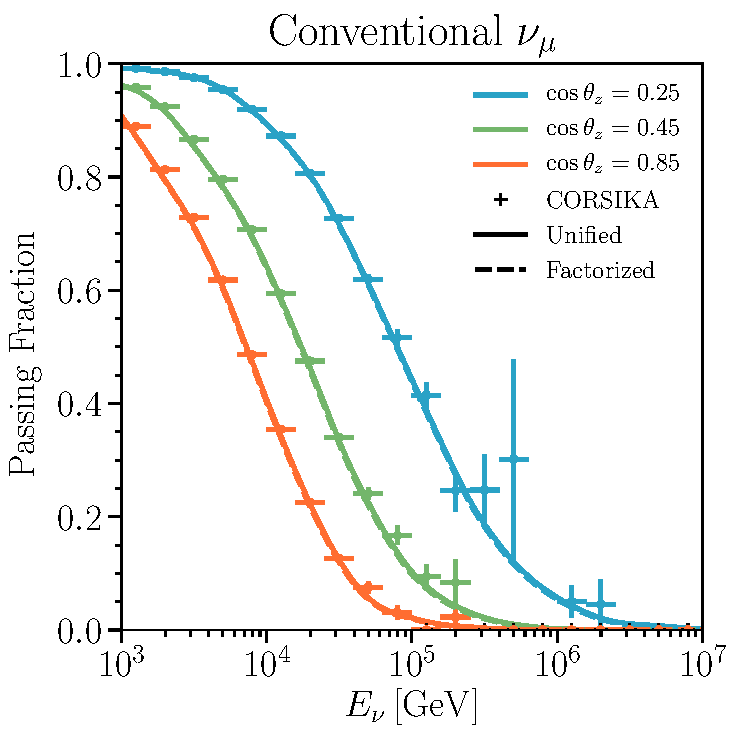
\includegraphics[width=0.45\linewidth]{results/passing_fractions_paper/fig/fig7_b_numu_convetional_unified_versus_factorized_with_corsika_sibyll_23}
	}
	\subfloat{
		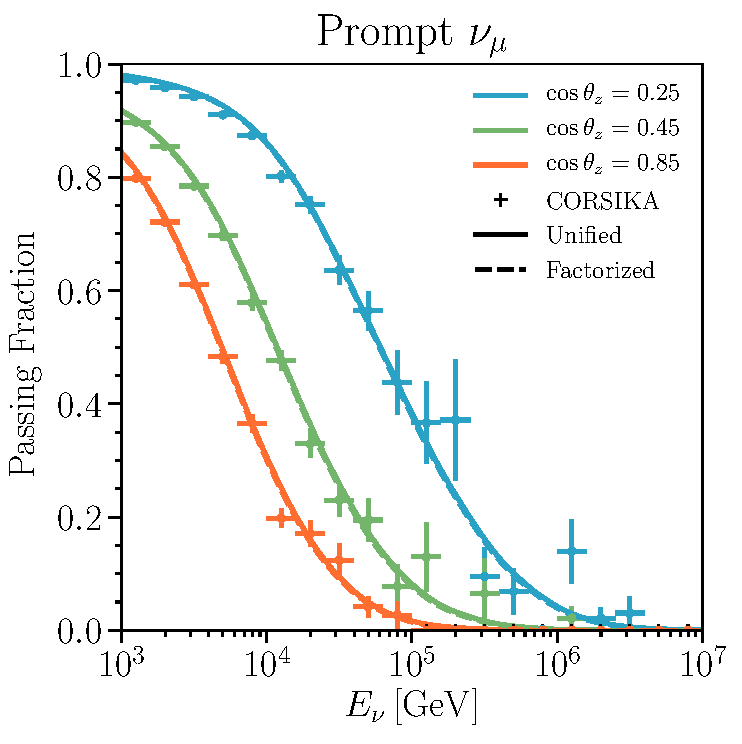
\includegraphics[width=0.45\linewidth]{results/passing_fractions_paper/fig/fig7_a_numu_prompt_unified_versus_factorized_with_corsika_sibyll_23}
	}
	\caption{\textbf{\textit{Passing fractions: differences between the unified and the factorized treatments for $\boldsymbol{\nu_\mu}$.}} Same as Fig.~\ref{fig:nue_passing-double-counting} regarding the approximations on the energy of the shower which gives rise to uncorrelated muons. Comparison of the unified treatment (solid), Eq.~(\ref{eq:GUE}), and the approximate treatment (dashed), Eq.~(\ref{eq:PGJKvS}), which factorizes the correlated and uncorrelated passing fractions. The result is driven by the correlated part.}
	\label{fig:nu-mu-unified-effect}
\end{figure}

The factorized and unified approaches are compared in Fig.~\ref{fig:nu-mu-unified-effect}, where one can see that the differences are negligible compared to the other effects discussed in this section.
The effect of the energy correction $\ECR-E_p$ is smaller for muon neutrinos than in the for electron neutrinos, shown in Fig.~\ref{fig:nue_passing-double-counting}, because for muon neutrinos $\Pzmsib$ is a much more dominant factor than $\Pzmproto$.
Note, for the uncorrelated part of the passing fraction, this subtraction is more important at higher energies, where the correlated contribution is very small.
Thus, the relative effect on the muon neutrino passing fraction is much smaller.
Finally, comparisons of the passing fractions calculated for muon neutrinos and muon antineutrinos are shown in Fig.~\ref{fig:nu-mu-neutrino-vs-antineutrino} and exhibit very good agreement with the Monte Carlo results, as in the case of electron neutrinos (Fig.~\ref{fig:nu-e-neutrino-vs-antineutrino}).

\begin{figure}
	\centering
	\subfloat{
		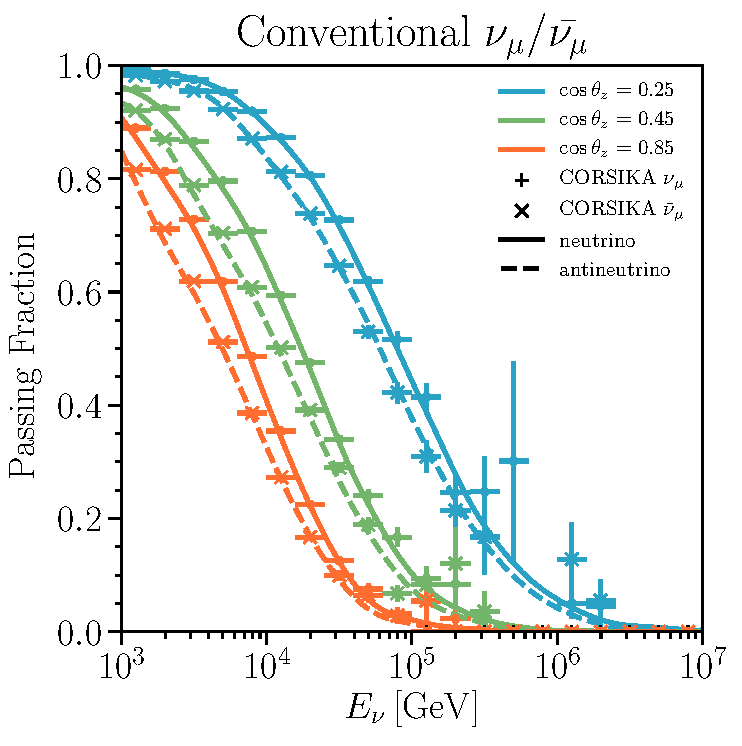
\includegraphics[width=0.45\linewidth]{results/passing_fractions_paper/fig/fig8_b_conventional_numu_versus_numubar_sibyll_23}
	}
	\subfloat{
		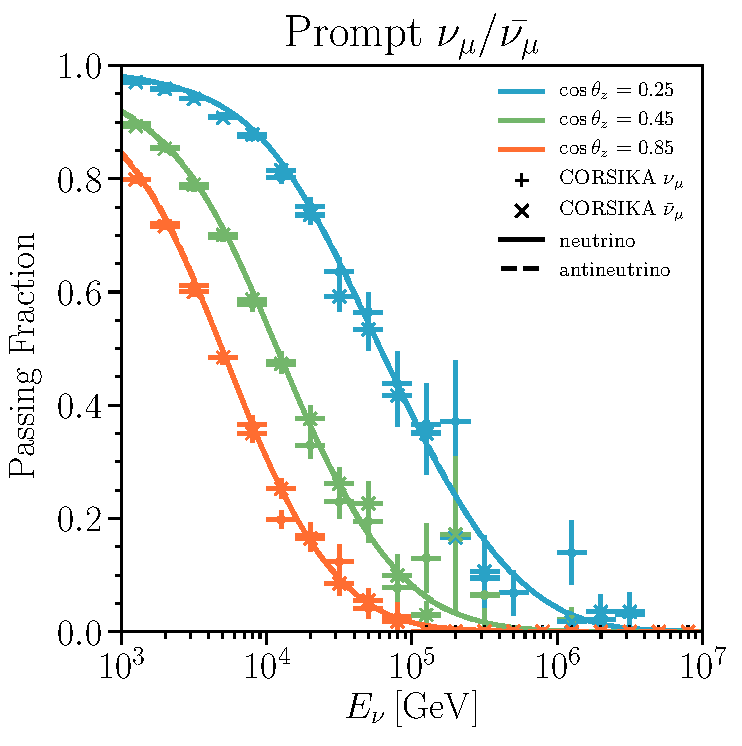
\includegraphics[width=0.45\linewidth]{results/passing_fractions_paper/fig/fig8_a_prompt_numu_versus_numubar_sibyll_23}
	}
	\caption{\textbf{\textit{Passing fractions: neutrinos versus antineutrinos.}} Same as Fig.~\ref{fig:nu-e-neutrino-vs-antineutrino} but for $\nu_\mu$ and $\bar\nu_\mu$. Note that for prompt neutrinos there are not differences between $\nu_\mu$ and $\bar\nu_\mu$.}
	\label{fig:nu-mu-neutrino-vs-antineutrino}
\end{figure}

A comparison of both the neutrino and antineutrino calculations to results from the CORSIKA simulation is shown in Fig.~\ref{fig:nu-mu-neutrino-vs-antineutrino}.
As with the calculation for electron neutrinos, the muon neutrino calculation shows excellent agreement with the air-shower simulations.

\subsubsection{Calculation improvements}

The calculation described in previous sections has many improvements with respect to earlier treatments.
A review of some earlier calculations will help us to examine the differences.

The first proposed calculation of the doing-going atmospheric neutrino suppression due to muons accounted only for sibling muons produced by the same parent meson as the neutrino.
This meant that the original calculation could only be applied to atmospheric muon neutrinos~\cite{Schonert:2008is}.
This original calculation used several analytic approximations, applicable to neutrinos produced in pion and kaon decays under the assumption of a power-;aw cosmic ray primary spectrum.
As described previously, the muon energy loss behavior for this calculation was treated using the median approximation, and the triggering probability modeled asa a Heaviside function.
These choices allowed analytic passing fractions to be derived.

In~\cite{Gaisser:2014bja} the analytic treatment was generalized to include muons from other branches of the shower, not associated with the production of the neutrino.
This generalization allowed the suppression to be computed for atmospheric electron neutrinos.
Analytic approximations were used to describe the average properties of muons from air showers.
In fact, the calculation in~\cite{Gaisser:2014bja} fit a parameterized $\bar N_{A,\mu}(\ECR, \theta_z)$ to the the results of CORSIKA simulation which sed SIBYLL 2.1 for conventional neutrinos and DMPJET-2.5 for prompt neutrinos.
The combination of these correlated and uncorrelated contributions led to Eq.~\ref{eq:PGJKvS}.
For these two calculations, the components were factorized and the $\ECR-E_p$ subtraction was not performed.
This led to an overestimation of the shower energy producing visible muons for the electron neutrino case.

The new approach, explained in the previous sections and developed in [] includes a full description of the cosmic ray primary spectrum and composition as well as the hadronic interactions that give rise to the parent particles and eventually muons and neutrinos.
This leads to the more accurate Eq.~\ref{eq:GUE} which is fully consistent between electron and muon neutrinos, although it must be calculated numerically.
Muon energy loss distributions are also fully accounted for in this treatment.
Critically, this approach uses numerical techniques instead of analytic approximations, opening the door for a wide array of modifications to the calculation.
These modifications can include: different detector configurations and responses, cosmic ray spectra, hadronic interaction models, atmospheric density models, and muon energy loss cross sections.
With these modifications the passing fraction calculation can be made consistent with the modern atmospheric neutrino flux calculations of $\MCEq$.

\begin{figure}
	\centering
	\subfloat{
		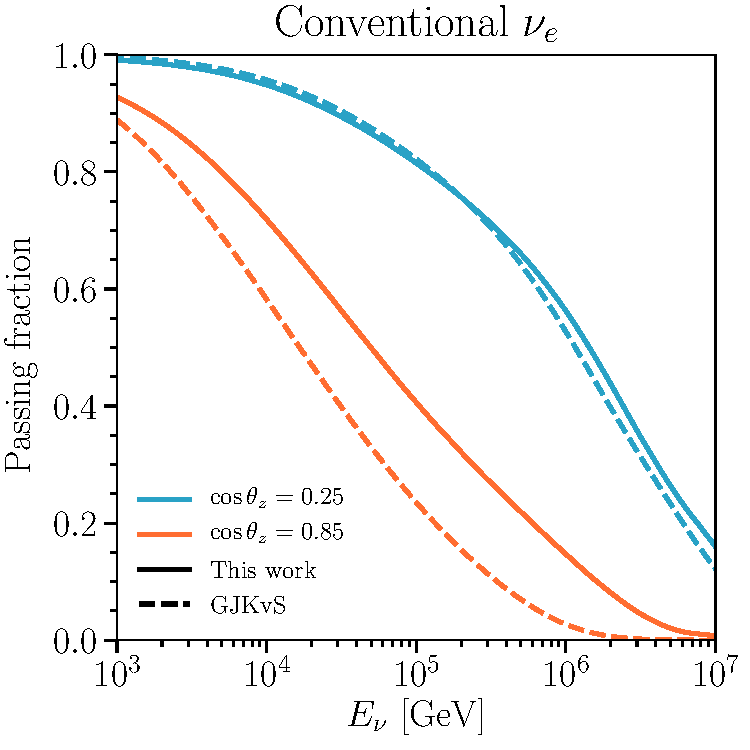
\includegraphics[width=0.45\linewidth]{results/passing_fractions_paper/fig/fig9_extsv_conv_nue}
	}
	\subfloat{
		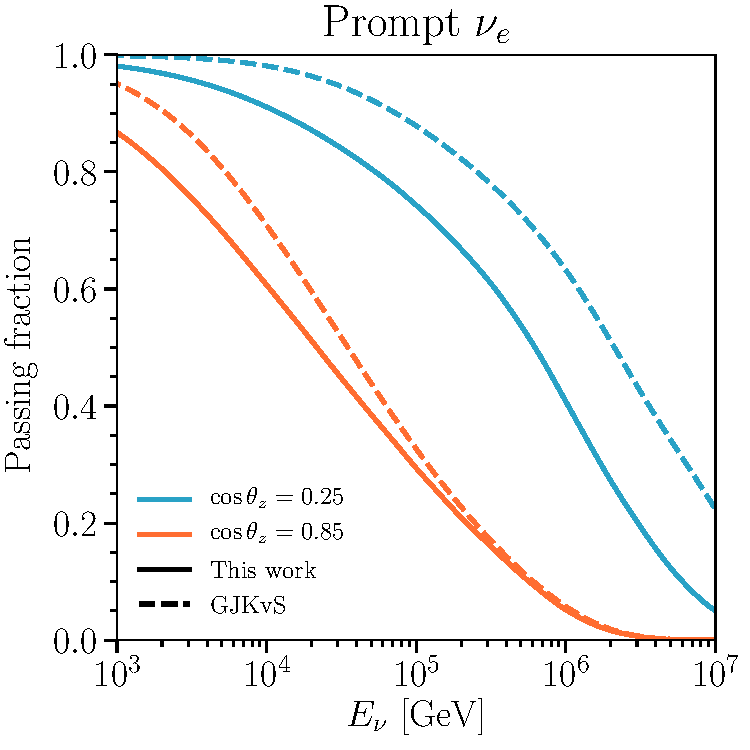
\includegraphics[width=0.45\linewidth]{results/passing_fractions_paper/fig/fig9_extsv_pr_nue}
	} \\[2ex]
	\subfloat{
		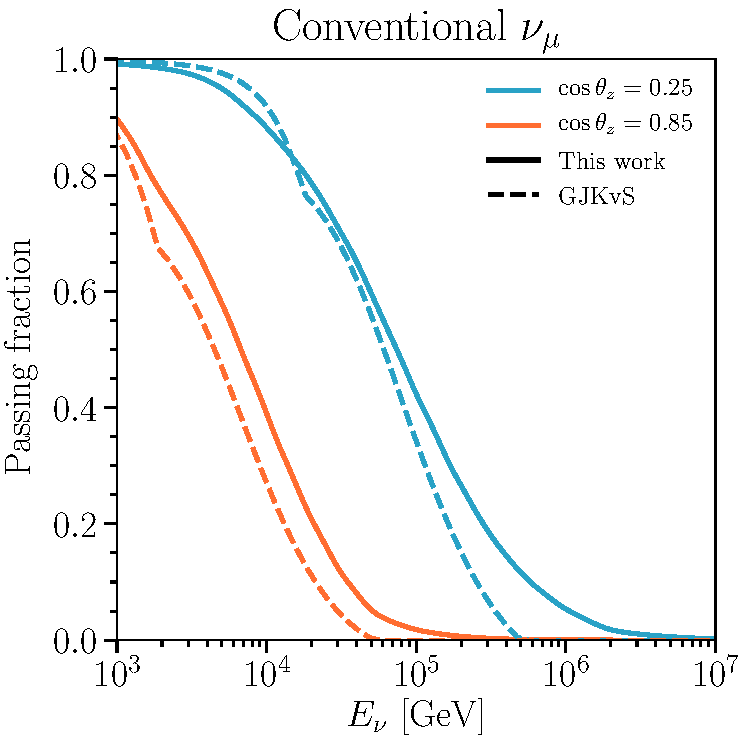
\includegraphics[width=0.45\linewidth]{results/passing_fractions_paper/fig/fig9_extsv_conv_numu}
	}
	\subfloat{
		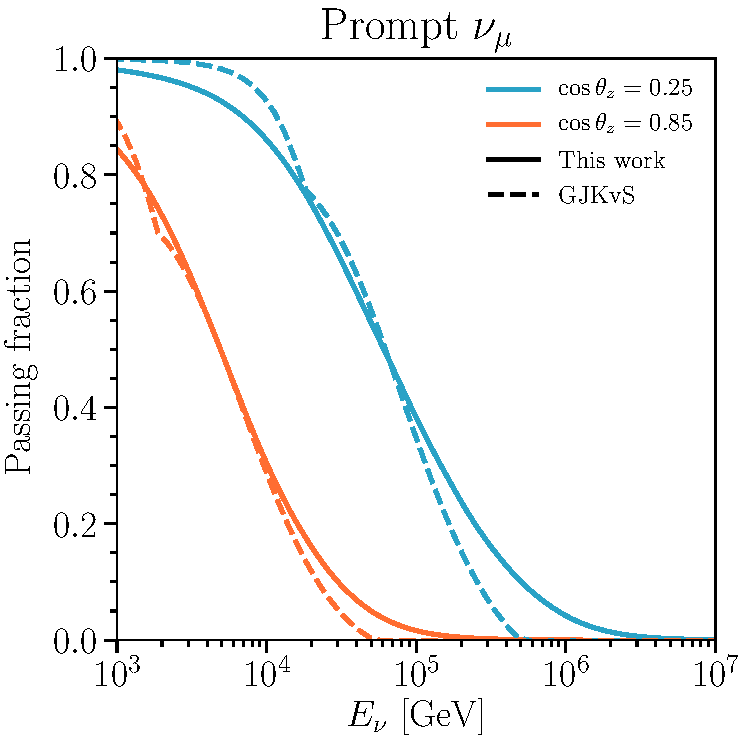
\includegraphics[width=0.45\linewidth]{results/passing_fractions_paper/fig/fig9_extsv_pr_numu}
	}
	\caption{\textbf{\textit{Passing fractions: comparison with previous work}}. Results are shown for two values of $\cos\theta_z =$ (from top to bottom): 0.25 (blue) and 0.85 (orange); with the calculation in this work (solid) and with that in Ref.~\cite{Gaisser:2014bja} (dashed). Our results are obtained with the H3a primary cosmic-ray spectrum~\cite{Gaisser:2011cc}, the SIBYLL~2.3c hadronic-interaction model~\cite{Riehn:2017mfm}, the MSIS-90-E atmosphere-density model at the South Pole on July 1, 1997~\cite{Labitzke:1985, Hedin:1991}, and assuming $d_{\rm det} = 1.95$~km in ice and $\Prob_{\rm light}(\Emf) = \Theta(\Emf - 1\,{\rm TeV})$. They include all of the effects discussed in previous sections, Eq.~(\ref{eq:GUE}). \textit{Top-left panel:} Conventional $\nu_e$ passing fraction. \textit{Top-right panel:} Prompt $\nu_e$ passing fraction. \textit{Bottom-left panel:} Conventional $\nu_\mu$ passing fraction. \textit{Bottom-right panel:} Prompt $\nu_\mu$ passing fraction.}
	\label{fig:nue-passing-comparison-old}
\end{figure}

Fig.~\ref{fig:nue-passing-comparison-old} shows a direct comparison between the new calculation and its predecessor~\cite{Gaisser:2014bja} for $\nu_e$ and $\nu_\mu$ from the conventional and prompt fluxes in two different directions.
In the more vertical direction, $\nu_e$ and $\nu_\mu$ passing fractions for the conventional flux show a large difference, where the newer calculation provides a higher passing fraction.
Two effects are important here, the muon range treatment and the energy of the uncorrelated shower branch.
Near the horizon these effects partially cancel, minimizing the difference between the two calculations, but that is not the case in the vertical direction.
The shoulder present in the older calculation shows the transition between the pion and kaon dominated production of neutrinos, however this is washed out by the more detailed muon range treatment of the new calculation.
The differences in the prompt $\nu_e$ curves are more difficult to interpret.
Comparisons of the muon range treatment and the energy subtraction for prompt $\nu_e$ would lead us to expect some small differences, but not quite of this magnitude.
One additional factor that could explain this, is the use of DPMJET-2.55 in the old calculation for prompt neutrinos; we see that DPMJET-2.55 gives larger passing fractions than SIBYLL 2.3c.
Differences in the prompt $\nu_\mu$ passing fractions are explained by the fact that~\cite{Gaisser:2014bja} applies the conventional $\nu_\mu$ passing fractions to prompt $\nu_\mu$.

\subsubsection{Calculation systematics}
The calculation outlines in these sections relies on a host of external information such as the cosmic ray flux, the physics governing decays and hadronic interactions, calculations of muon energy loss cross sections, and the detector response.
In this section, a few of these potential sources of uncertainty are examined.

\paragraph{Muon Energy Losses}
Muons lose energy in a medium through three processes: ionization losses, $e^+e^-$ pair production, bremsstrahlung, and photo-nuclear interactions.
Below $\sim\SI{1}\TeV$ losses are dominated by ionization.
Whereas, at higher energies the radiative processes dominate.
In order of importance these are pair production, bremsstrahlung, and photo-nuclear interactions.
Above $\sim\SI{10}\PeV$ photo-nuclear interactions are comparable to bremsstrahlung~\cite{Chirkin:2004hz}.
These processes are well understood up to $\sim\SI{10}\TeV$ in muon energy, above which the photo-nuclear interactions dominate the uncertainty in the cross section.

The photo-nuclear cross section used in MMC/PROPOSAL by default uses a data-driven parameterization of the proton structure function in a deep-inelastic scattering (DIS) formalism~\cite{Abramowicz:1991xz, Abramowicz:1997ms}.
This formalism includes contributions from both soft (non-perturbative) and hard (perturbative) physics~\cite{Dutta:2000hh}.
Another approach describes the cross section with a generalized vector dominance model for the soft component~\cite{Bezrukov:1981ci} and a framework of the color dipole moment for the hard component~\cite{Bugaev:2002gy, Bugaev:2003sw}.

Without appropriate measurements and the corresponding data-derived uncertainties the cross section uncertainty can be examined by comparing the two calculation approaches.
At the energies relevant for the passing fraction calculation the default cross sections are slightly lower, resulting in smaller passing fractions as more muons can reach the detector with higher energy.
These differences in the cross section result in a maximum difference of 0.01 for the passing fractions.

\paragraph{Primary Cosmic Ray Spectra}
Previously shown comparisons all assume the Hillas-Gaisser three population model (H3a)~\cite{Gaisser:2011cc}.
This model considers five different nuclei mass groups with three populations.
These cut off at a characteristic rigidity.
Other models for the cosmic ray primary flux have been proposed, and current measurements leave a considerable amount of uncertainty in the energy regime relevant for the passing fractions.

A second model, GST-4gen~\cite{Gaisser:2013bla}, has a lower cutoff for the first two populations which also have correspondingly harder spectra.
While the third population is iron-only above the spectrum ankle.
A fourth proton-only component is included to obtain better agreement with shower depth data around $\SI{1}\EeV$.
However, this proton-iron composition is somewhat in tension with data from Auger~\cite{Abraham:2010yv, Aab:2014aea}.

A third model, ZS~\cite{Zatsepin:2006ci}, has three components derived from specific astrophysical sources.
The lowest energy population comes from the expanding shells of supernovae remnants.
The middle energy component comes from isolated supernovae and their interaction with the interstellar medium.
Finally, the high energy component comes from massive star supernovae explosions and their interaction with their own stellar wind.
This last process produces a very heavy composition.

\begin{figure}[h!]
	\centering
	\subfloat{
		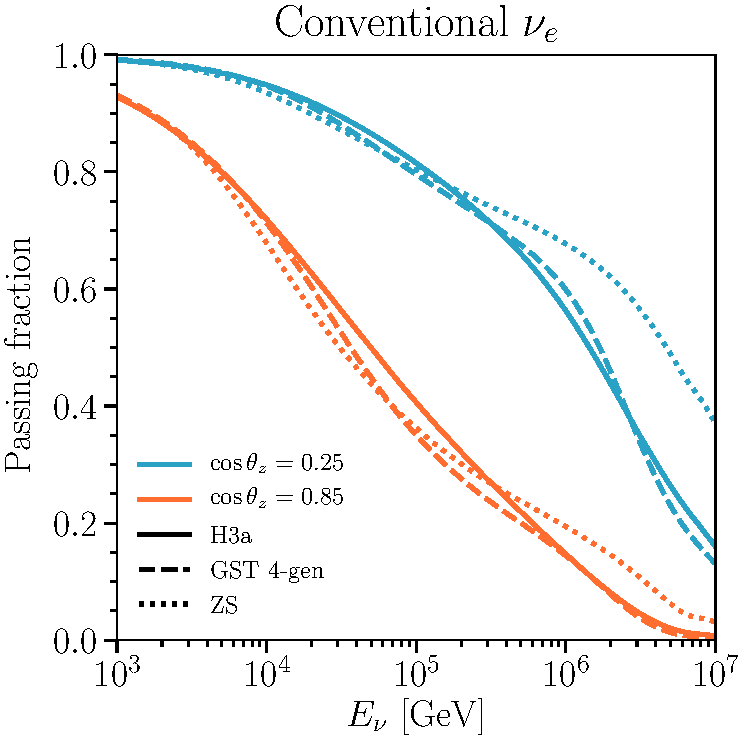
\includegraphics[width=0.45\linewidth]{results/passing_fractions_paper/fig/fig10_pmodels_conv_nue}
	}
	\subfloat{
		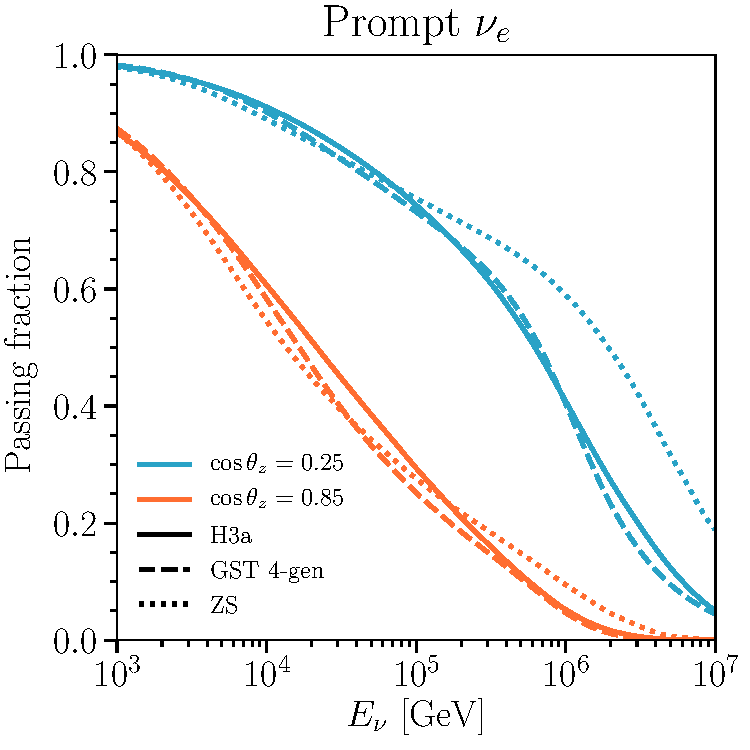
\includegraphics[width=0.45\linewidth]{results/passing_fractions_paper/fig/fig10_pmodels_pr_nue}
	}\\[2ex]
	\subfloat{
		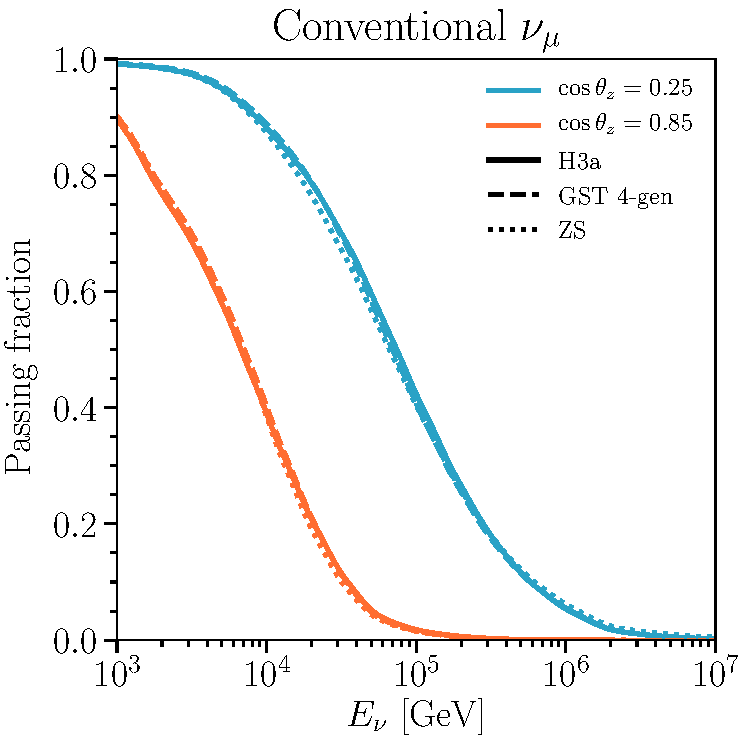
\includegraphics[width=0.45\linewidth]{results/passing_fractions_paper/fig/fig10_pmodels_conv_numu}
	}
	\subfloat{
		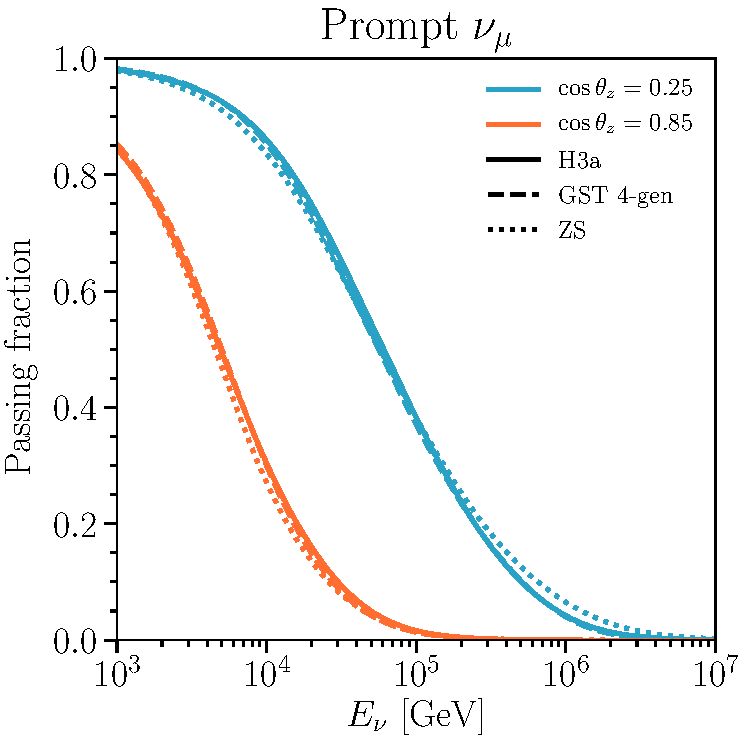
\includegraphics[width=0.45\linewidth]{results/passing_fractions_paper/fig/fig10_pmodels_pr_numu}
	}
	\caption{\textbf{\textit{Passing fractions: effect of primary cosmic-ray spectrum}}. Results are shown for two values of $\cos\theta_z$ (from top to bottom): 0.25 (blue) and 0.85 (orange); for four CR models: Hillas-Gaisser H3a~\cite{Gaisser:2011cc} (solid), Gaisser, Stanev and Tilav (GST 4-gen)~\cite{Gaisser:2013bla} (dashed) and Zatsepin-Solkolskaya (ZS)~\cite{Zatsepin:2006ci} (dotted).
		\textit{Top-left panel:} Conventional $\nu_e$ passing fraction. \textit{Top-right panel:} Prompt $\nu_e$ passing fraction. \textit{Bottom-left panel:} Conventional $\nu_\mu$ passing fraction. \textit{Bottom-right panel:} Prompt $\nu_\mu$ passing fraction.}
	\label{fig:nue-cr-model-effect} \vspace{1.5cm}
\end{figure}

These three models are compared by their effect on the passing fraction calculations in Fig.~\ref{fig:nue-cr-model-effect}.
The largest differences are for the $\nu_e$ passing fractions, which differ between models by less than 0.05 except when comparing the ZS model above $\SI{e6}\GeV$.
This can be understood as a consequence of the ZS model being designed only to describe the cosmic ray flux up to $\SI{e8}\GeV$, meaning the ZS neutrinos flux predictions may not be accurate above $\SI{e6}\GeV$.
The muon neutrinos passing fractions have much smaller variations between models.
This is likely a result fo the sister muons dominating the passing fraction calculation, meaning that the population of showers from which the neutrino may have originated is a subdominant effect.
The level of variation seen between these models represents a non-negligible uncertainty in the passing fractions for electron neutrinos, but is small for muon neutrinos.
However, this level of uncertainty alone is likely to be smaller than the statistical uncertainties currently present for the HESE sample.

Here a bracketing approach was used to examine the uncertainties, and models chosen to express a range of possibilities currently allowed by experimental measurements.
But this is not a full accounting of the cosmic ray flux uncertainties.
The measurement uncertainties can be accounted for in a more satisfactory manner with a non-parametric fit with sufficient degrees of freedom to the available cosmic-ray data.
For any point in the parameter space of this fit both the neutrino flux and passing fraction can be computed to provide an expectation for the ``apparent'' neutrino flux.
By directly using estimates from this fit and allowing the cosmic ray model to vary in a fit of neutrino data the uncertainties can be treated appropriately.
This method has some computational challenges as it is not feasible to run the necessary MCEq calculations each time a different point in the parameter space is tested.
However, there are some optimizations that can be found by carefully examining the basis functions used for the different cosmic ray populations and pre-computing or caching information where applicable.
Such a treatment is not used for the HESE 7.5 year analysis, but may prove to be useful for future analyses that combine multiple samples with more than 10 years of data.

\paragraph{Hadronic Interaction Models}
The muons and neutrinos relevant for this calculation are produced in high energy extensive air showers, the development of which is governed by hadronic interaction physics.
However, these showers and hadronic interactions occur at energies that are orders of magnitude beyond what is accessible to collider experiments where these interactions can be measured.
Thus, our predictions for how these showers develop depends heavily on hadronic models that may are tuned to collider data but are extrapolations at the energies we are concerned with.

\begin{figure}[h!]
	\centering
	\subfloat{
		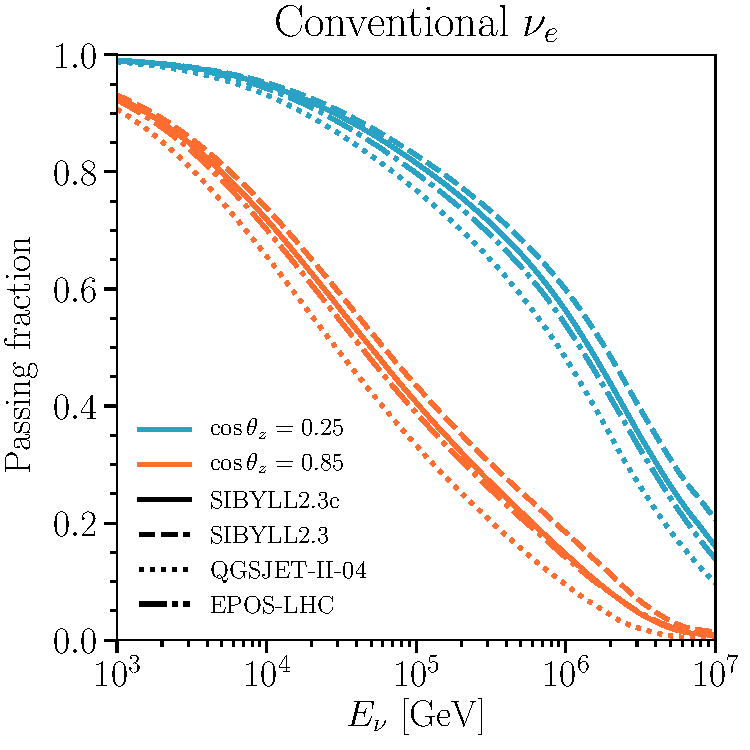
\includegraphics[width=0.45\linewidth]{results/passing_fractions_paper/fig/fig11_hadrs_conv_nue}
	}
	\subfloat{
		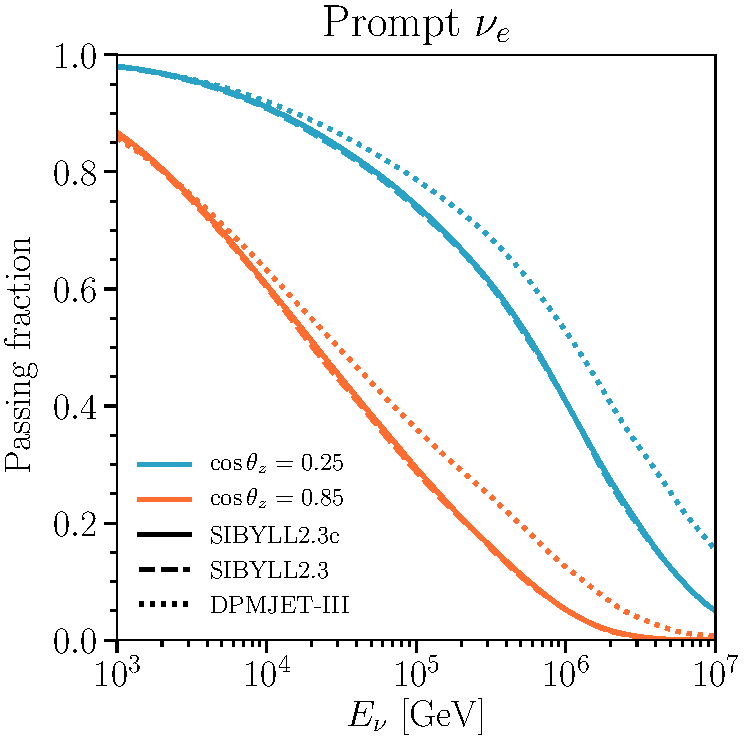
\includegraphics[width=0.45\linewidth]{results/passing_fractions_paper/fig/fig11_hadrs_pr_nue}
	}\\[2ex]
	\subfloat{
		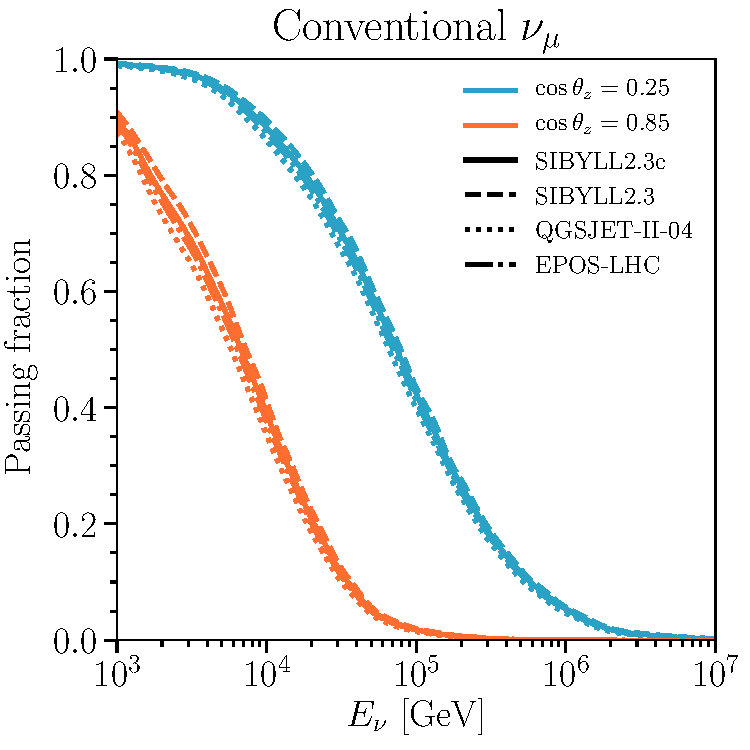
\includegraphics[width=0.45\linewidth]{results/passing_fractions_paper/fig/fig11_hadrs_conv_numu}
	}
	\subfloat{
		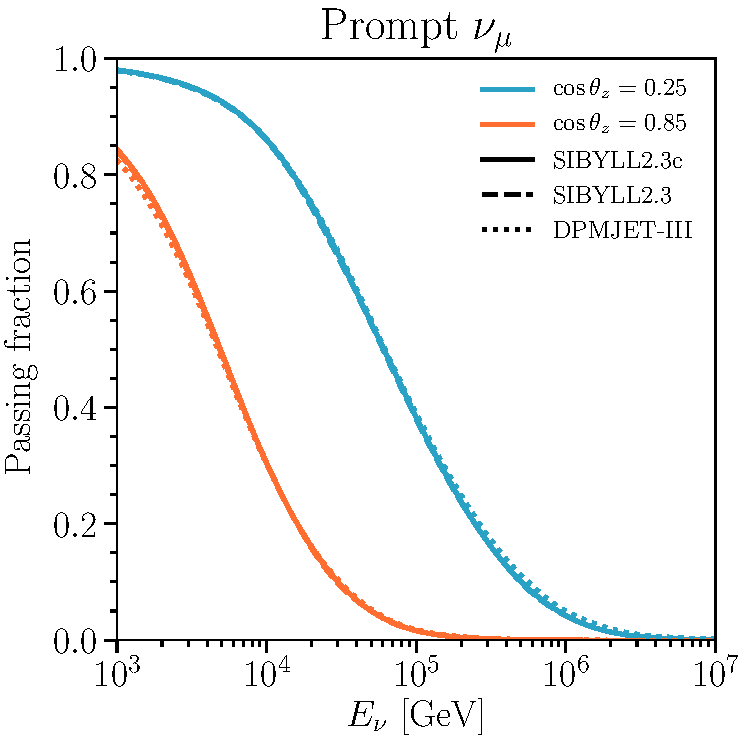
\includegraphics[width=0.45\linewidth]{results/passing_fractions_paper/fig/fig11_hadrs_pr_numu}
	}
	\caption{\textbf{\textit{Passing fractions: effect of hadronic-interaction model}}. Results are shown for two values of $\cos\theta_z$ (from top to bottom): 0.25 (blue) and 0.85 (orange); for different hadronic-interaction models: SIBYLL~2.3c~\cite{Riehn:2017mfm} (solid), SIBYLL~2.3~\cite{Engel:2015dxa, Riehn:2015oba} (dashed), QGSJET-II-04~\cite{Ostapchenko:2010vb} (dotted in left panel), EPOS-LHC~\cite{Pierog:2013ria} (dash-dotted in left panel) and DPMJET-III\cite{Roesler:2000he} (dotted in right panel).
		\textit{Top-left panel:} Conventional $\nu_e$ passing fraction. \textit{Top-right panel:} Prompt $\nu_e$ passing fraction. \textit{Bottom-left panel:} Conventional $\nu_\mu$ passing fraction. \textit{Bottom-right panel:} Prompt $\nu_\mu$ passing fraction.} \vspace{1cm}
	\label{fig:nue-hadronic-model-effect}
\end{figure}

Figure~\ref{fig:nue-hadronic-model-effect} shows a comparison of the passing fractions computed assuming four different hadronic interaction models.
A detailed discussion of the differences between these models can be found in Section IV.C of~\cite{Arguelles:2018awr}.
For electron neutrinos there are non-negligible differences in the passing fractions, but the variation is again small for muon neutrinos.

\paragraph{Depth and Surrounding Medium}
In these sections a depth of $\SI{1.95}\km$ has been assumed to model the veto effects at the center of the IceCube detector.
However, IceCube and other neutrino detectors are large enough that the change in depth from top to bottomo significantly changes the overburden for a neutrino of a given zenith angle.
Increases in the overburden significantly reduce the power of the veto, as muons that reach the detector are fewer and less energetic.
As a benchmark, we can examine the passing fractions assuming a depth of $\SI{3.5}\km$, corresponding to the depth of KM3NeT-Italy, and also compare differences between ice and water.

\begin{figure}[h!]
	\centering
	\subfloat{
		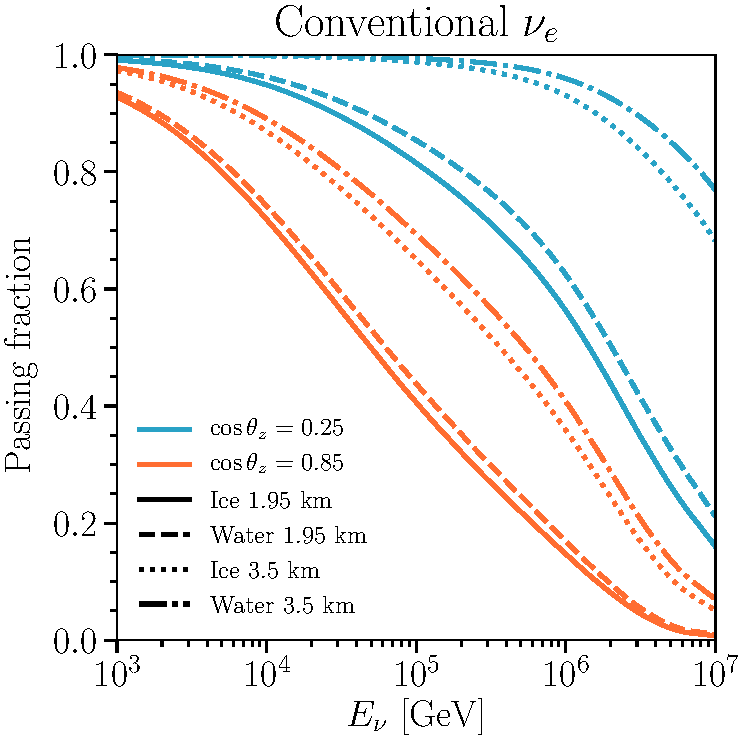
\includegraphics[width=0.45\linewidth]{results/passing_fractions_paper/fig/fig13_medium_conv_nue}
	}
	\subfloat{
		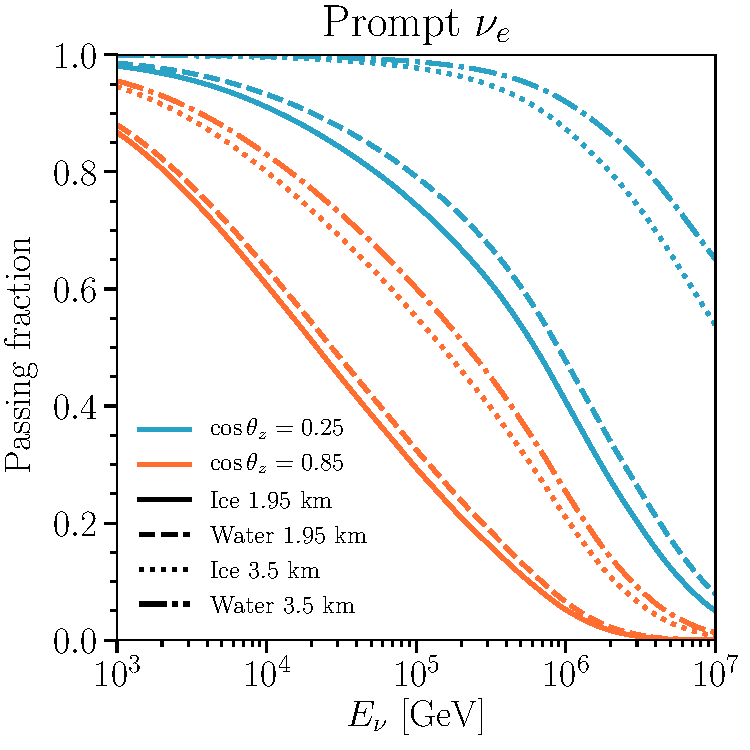
\includegraphics[width=0.45\linewidth]{results/passing_fractions_paper/fig/fig13_medium_pr_nue}
	}\\[2ex]
	\subfloat{
		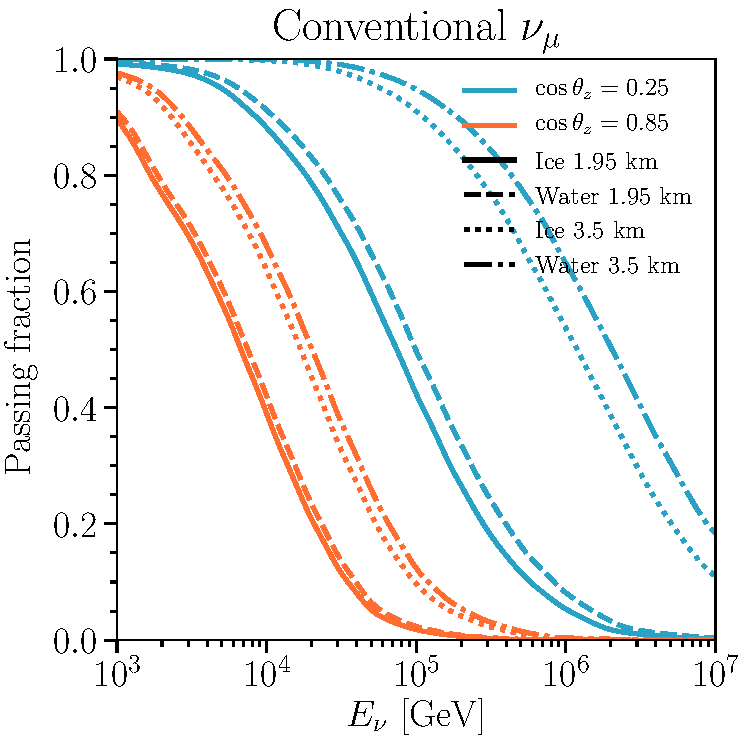
\includegraphics[width=0.45\linewidth]{results/passing_fractions_paper/fig/fig13_medium_conv_numu}
	}
	\subfloat{
		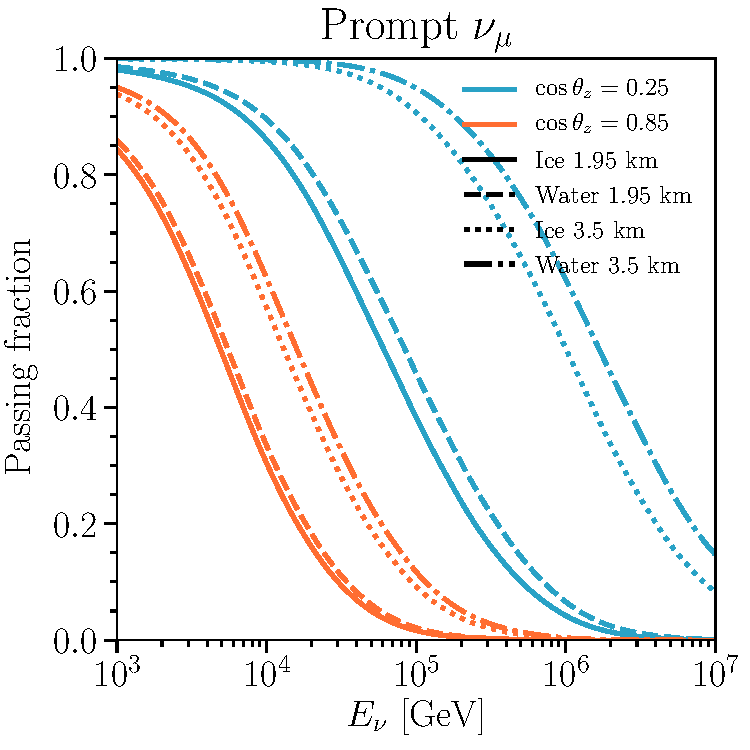
\includegraphics[width=0.45\linewidth]{results/passing_fractions_paper/fig/fig13_medium_pr_numu}
	}
	\caption{\textbf{\textit{Passing fractions: effect of depth/medium}}. Results are shown for two values of $\cos\theta_z$ (from top to bottom): 0.25 (blue) and 0.85 (orange); for two depths: $d_{\rm det} = 1.95$~km (solid and dashed) and $d_{\rm det} = 3.5$~km (dotted and dash-dotted); and for two different media: ice (solid and dotted) and water (dashed and dot-dashed). \textit{Top-left panel:} Conventional $\nu_e$ passing fraction. \textit{Top-right panel:} Prompt $\nu_e$ passing fraction. \textit{Bottom-left panel:} Conventional $\nu_\mu$ passing fraction. \textit{Bottom-right panel:} Prompt $\nu_\mu$ passing fraction.} \vspace{1.5cm}
	\label{fig:medium-effect}
\end{figure}

Figure~\ref{fig:medium-effect} shows these comparisons.
It is notable that the differences between water and ice are non-negligible but much less dramatic than the effect of depth.
As expected, the effect of the surrounding medium is also more pronounced near the horizon where the change in effective overburden is larger.
The increased depth results in a significantly larger passing fraction, greatly reducing the power of veto techniques.
It is therefore important to model the depth of events to accurately determine their passing probability.
Depth is also an important consideration when evaluating the sensitivity of different neutrino detectors to the astrophysical flux.

\paragraph{Detector Response}
The probability for a muon to trigger the veto, $\Prob_{\rm light}$, encapsulates the detector response that is relevant for the passing fraction calculation.
So far in this discussion all the passing fractions have been computed with a $\SI{1}\TeV$ threshold Heaviside $\Prob_{\rm light}$.
While the Heaviside parameterization is simple, the real detector response is certainly more complex.
The particular form of $\Prob_{\rm light}$ will depend on the particulars of the implemented veto.
To get a feel for these differences and the uncertainty that detector response modeling could introduce we look at a few different $\Prob_{\rm light}$ functions.

\begin{figure}[h!]
	\centering
	\subfloat{
		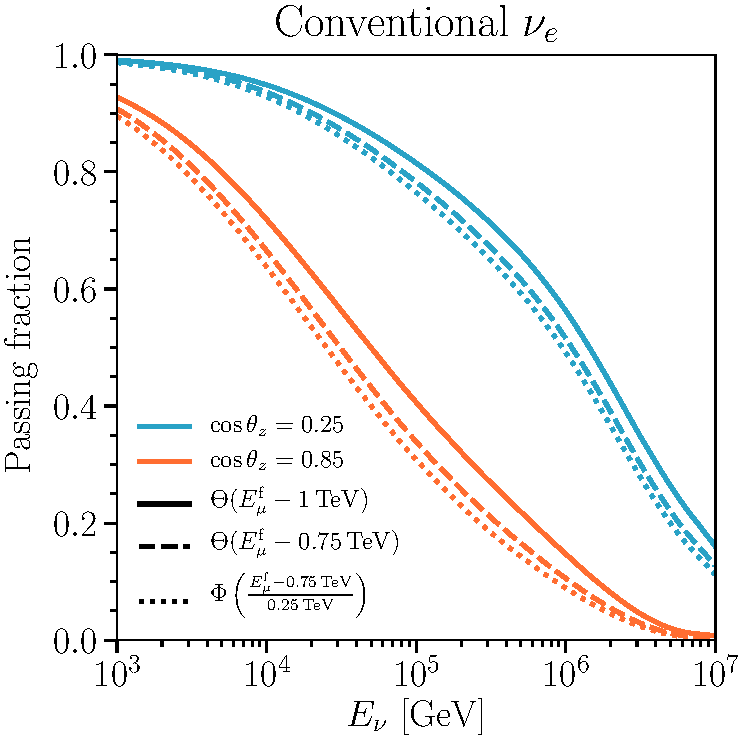
\includegraphics[width=0.45\linewidth]{results/passing_fractions_paper/fig/fig14_pls_conv_nue}
	}
	\subfloat{
		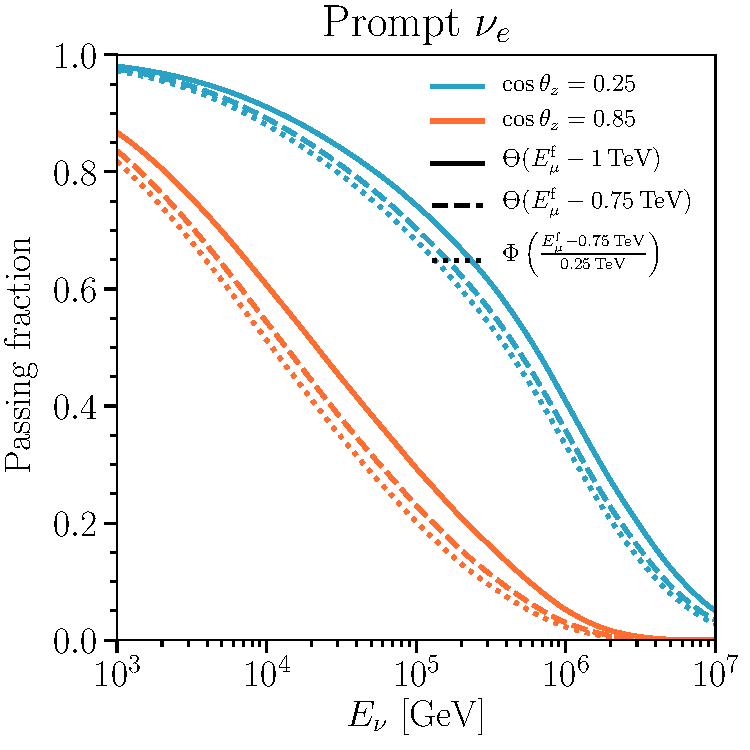
\includegraphics[width=0.45\linewidth]{results/passing_fractions_paper/fig/fig14_pls_pr_nue}
	}\\[2ex]
	\subfloat{
		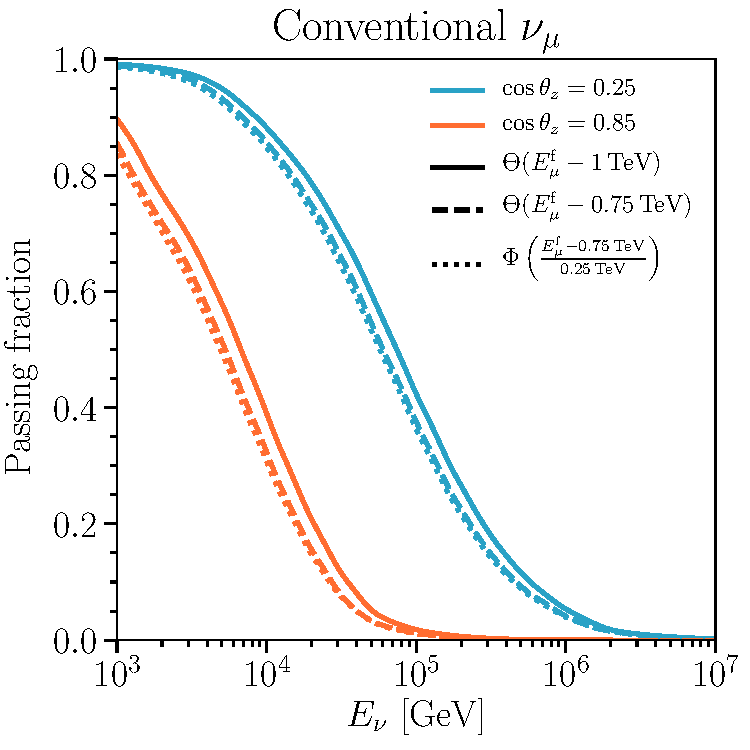
\includegraphics[width=0.45\linewidth]{results/passing_fractions_paper/fig/fig14_pls_conv_numu}
	}
	\subfloat{
		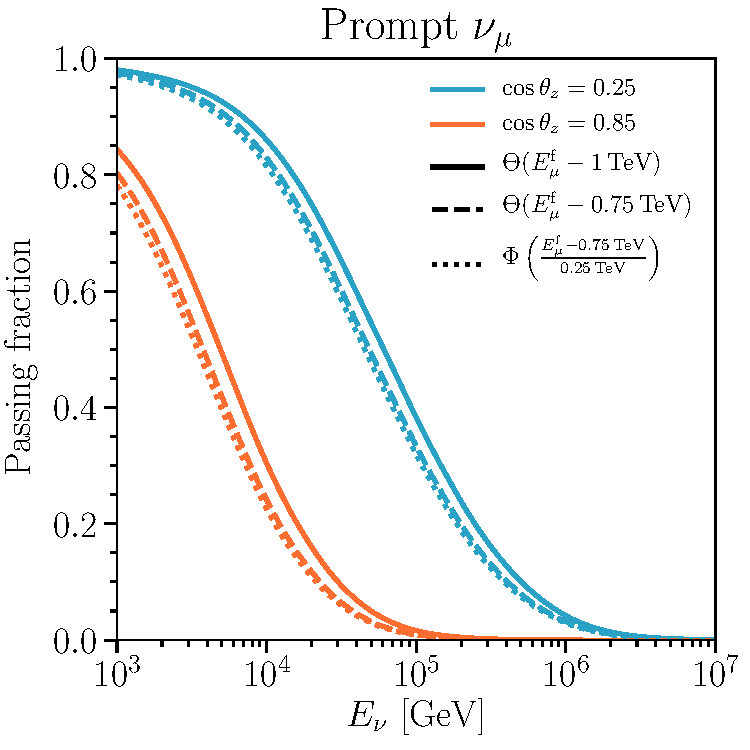
\includegraphics[width=0.45\linewidth]{results/passing_fractions_paper/fig/fig14_pls_pr_numu}
	}
	\caption{\textbf{\textit{Passing fractions: effect of $\boldsymbol{\Prob_{\rm light}}$}}. Results are shown for two values of $\cos\theta_z$ (from top to bottom): 0.25 (blue) and 0.85 (orange); for three different $\Prob_{\rm light}(\Emf)$: a Heaviside with a muon threshold at 1~TeV, $\Theta\left(\Emf - 1 \, {\rm TeV}\right)$ (solid), a Heaviside with a muon threshold at 0.75~TeV, $\Theta\left(\Emf - 0.75 \, {\rm TeV}\right)$ (dashed) and a sigmoid $\Phi\left(\left(\Emf - 0.75 \, {\rm TeV}\right)/0.25 \, {\rm TeV}\right)$ (dotted). \textit{Top-left panel:} Conventional $\nu_e$ passing fraction. \textit{Top-right panel:} Prompt $\nu_e$ passing fraction. \textit{Bottom-left panel:} Conventional $\nu_\mu$ passing fraction. \textit{Bottom-right panel:} Prompt $\nu_\mu$ passing fraction.} \vspace{1.5cm}
	\label{fig:nue-plight-effect}
\end{figure}

With straightforward veto implementations a smooth, monotonic, threshold-like behavior is expected.
This can be understood as a consequence of three factors: cuts on observable parameters, fluctuations in observed light, and the positive correlation between muon energy and light emission.
The cuts on observable parameters introduce the threshold behavior, choosing to accept and reject events that fall into different regions of the observable parameter space.
However, this hard threshold is smoothed out by fluctuations in the observable parameters.
Stochastic energy losses of the muons mean that the emitted light near the veto can vary wildly for identical muons; further variation is caused by photon scattering and the quantum efficiency of the detector PMTs.
The Heaviside function models this threshold behavior but transitions too sharply represent a realistic detector response.
An alternative is to use a sigmoid to model the smooth transition, in this case a logistic function is a reasonable choice.
Figure~\ref{fig:nue-plight-effect} shows the passing fractions for three variations of the $\Prob_{\rm light}$ function, a Heaviside with $\SI{1}\TeV$ threshold, a Heaviside with $\SI{0.25}\TeV$ threshold, and finally a logistic function with a $\SI{0.25}\TeV$ threshold and $1/\SI{0.25}\TeV$ growth parameter.
A reduction in the Heaviside function threshold produces a reduction of the passing fraction as expected.
The change from Heaviside to sigmoid produces a smaller reduction, although this comparison of the effect's magnitude is arbitrary.
Although the change to muon neutrino passing fractions is smaller than that for electron neutrinos, this is the largest change in the muon neutrino passing fraction for a fixed detector geometry.
We should stress the importance of correctly modeling the detector response to muons as it will significantly affect the passing fractions for both flavors.

\subsubsection{HESE passing fractions}
In this approach the neutrino properties are known from simulation, and it is sought to average over all the potential properties of the cosmic ray air showers from which the neutrino could have been produced in.
Ideally this average over air shower properties should be computed for each neutrino position, direction, and energy because the detector response can vary with all six of these parameters.
However, not all of these properties are used directly in the analysis nor does the detector response depend equally on all of these parameters.
For this reason when performing the calculation of the efficiency, only the neutrino energy, zenith angle, and depth upon intersection with the detector are considered.
Other properties of the neutrino are averaged over.
Additionally, in the characterization of the detector response to muons, only dependence on the muon energy and depth are considered.
Thus, the computed passing fraction depends on the neutrino energy, the zenith angle, and the incident depth in the detector.
However, the detector response and neutrino properties can be factorized so that the problem may be discussed more generally.
In previous analyses, the passing fractions were calculated using an extension of the method described in~\cite{Schonert:2008is} and bounded at $\SI{10}\percent$; details of the method are provided in~\cite{Aartsen:2013jdh}.
Cosmic ray simulations remain a computationally prohibitive way of accounting for the effects of accompanying muons, so we still rely on calculations of the average passing rate.
In this analysis, we use the new calculation described above and in~\cite{Arguelles:2018awr} that allows for different cosmic-ray and hadronic models to be used; more importantly for this analysis any parameterization of the detector veto response to muons can be used in the calculation, as opposed to just an energy threshold.
This capability allows us to more accurately model the detector response to atmospheric neutrinos.
In \reffig{fig:P_light} we show the probability that a muon will pass the veto as a function of the true muon incident energy for different detector depths.

% Plot of p_light
\begin{figure}
	\centering
	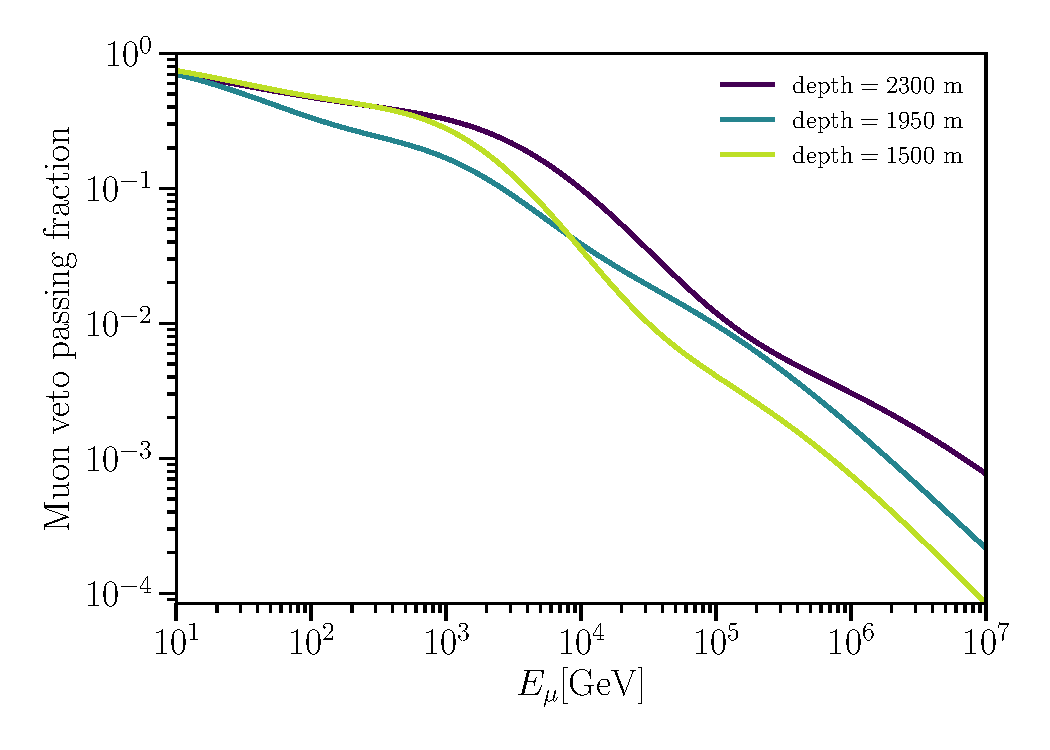
\includegraphics[width=\linewidth]{results/HESE_Final_Paper/figures/plight}
	\internallinenumbers
	\caption{\textbf{\textit{Muon veto passing fraction.}} Each line shows the fraction of muons of a given energy at the detector edge, $E_\mu$, that pass without triggering the veto when entering the detector at a particular depth.
		Three depths are shown: 1500, 1950, and 2300 meters from the surface; with lines of darkening color as the depth increases.
		The veto efficiency increases with the muon energy.
		Differences at various depths are due to the changing ice properties, and varying acceptance as a function of depth due to the asymmetric structure of the veto region.
		At all depths a sigmoid function is fit to the results of muon simulation.
		Above $\sim\SI{100}\TeV$ the passing fraction is extrapolated.}\label{fig:P_light}
\end{figure}

Using the muon passing fractions in \reffig{fig:P_light} as input and the \nuveto{} code provided in~\cite{Arguelles:2018awr} the atmospheric passing fraction is calculated for each component and flavor using the Hillas-Gaisser H3a~\cite{Gaisser:2013bla,Gaisser:2011cc,Hillas:2006ms} model for the incident cosmic-ray spectra and SIBYLL2.3c~\cite{Riehn:2017mfm} for the hadronic interactions in the air shower.
Switching to passing fractions derived from alternative cosmic-ray and hadronic interaction models has sub-leading effects in determination of the astrophysical flux~\cite{Arguelles:2018awr}.
Effects of these systematics were studied by repeating the analysis for different passing fractions that arise from a given combination of cosmic-ray spectrum and hadronic model for a variety of spectra and models that are available in the literature.
We found that the inclusion of these effects in addition to other discrete ice choices mentioned later in \refsec{sec:detector_systematics} increases the reported uncertainty of the astrophysical parameters by at most $\SI{20}\percent$ with respect to errors computed without these effects.
For this reason, these effects are not included in the analysis and are not reflected in the reported errors of any model parameters.
In \reffig{fig:passingfraction} we show the passing fractions for the conventional and prompt neutrino components.
In these figures the left, center, and right panels correspond to $\cos\theta_z$ values of 0.1, 0.3, and 0.9 respectively; the solid lines correspond to muon neutrinos and the dashed lines to electron neutrinos.
From the progression of the panels from left to right, one can see the passing fractions become smaller as one approaches vertical directions.
Vertical muons have the highest probability of reaching the detector, as the overburden they pass through is the smallest.
Though not shown in this figure, the conventional passing fractions differ from neutrinos to anti-neutrinos, see~\cite{Arguelles:2018awr} for details; the appropriate passing fractions are used in this analysis.
\reffigs{fig:conventional_distribution}{fig:prompt_distribution} show the distributions of conventional and prompt neutrinos respectively after this correction is applied.
This reduction in atmospheric background accounts for much of the sensitivity of this analysis to the astrophysical neutrino flux, as the observed down-going atmospheric fluxes in IceCube would otherwise be comparable in magnitude and remain similar in their angular distribution.
This is best seen when comparing the atmospheric fluxes before and after the veto to the measured astrophysical flux as shown in \reffig{fig:neutrino_spectrum}.

% Plot of the passing fraction for different heights (one line per height) (one panel for each costh [3 values])
\begin{figure*}
	\centering
	\subfloat{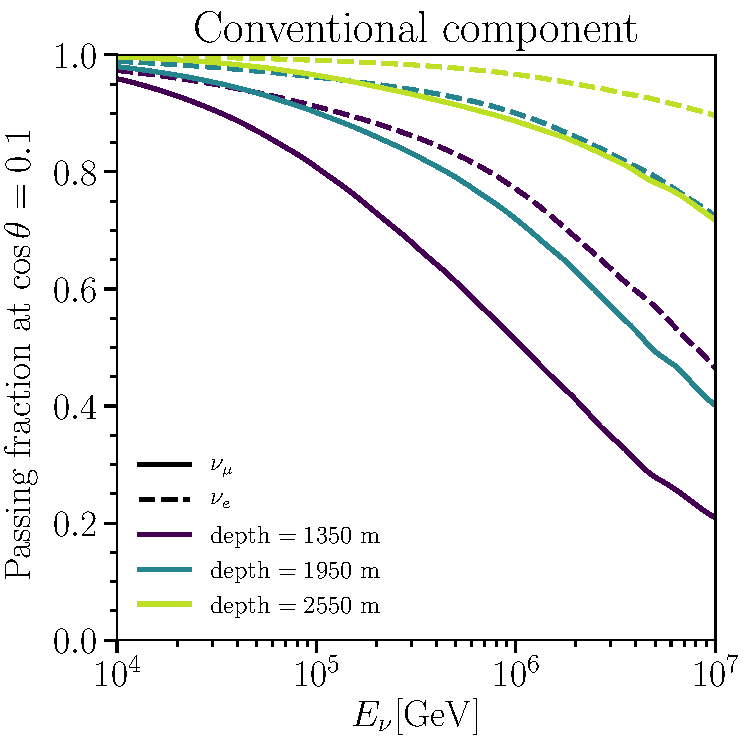
\includegraphics[width=0.3\linewidth]{results/HESE_Final_Paper/figures/conv_0_1_passing_fraction}}
	\subfloat{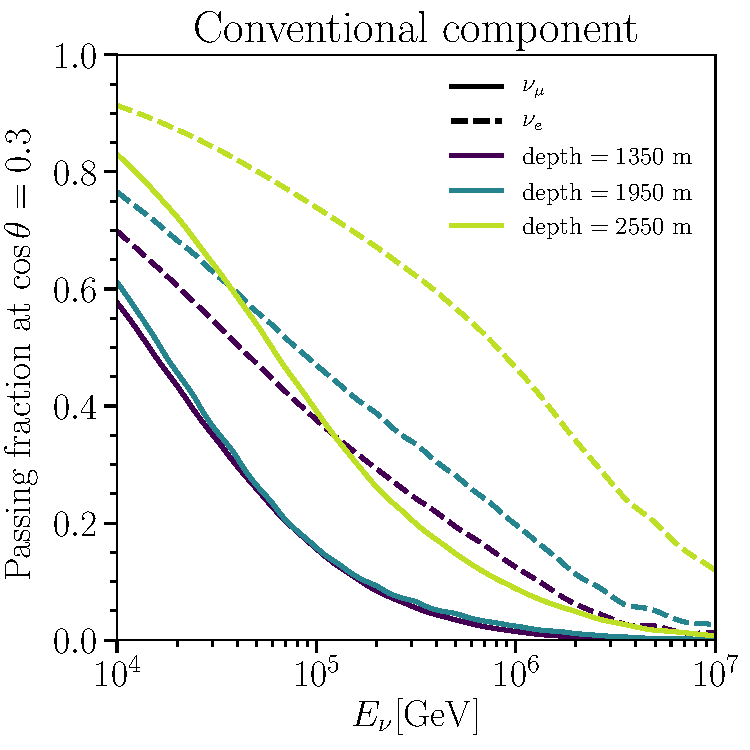
\includegraphics[width=0.3\linewidth]{results/HESE_Final_Paper/figures/conv_0_3_passing_fraction}}
	\subfloat{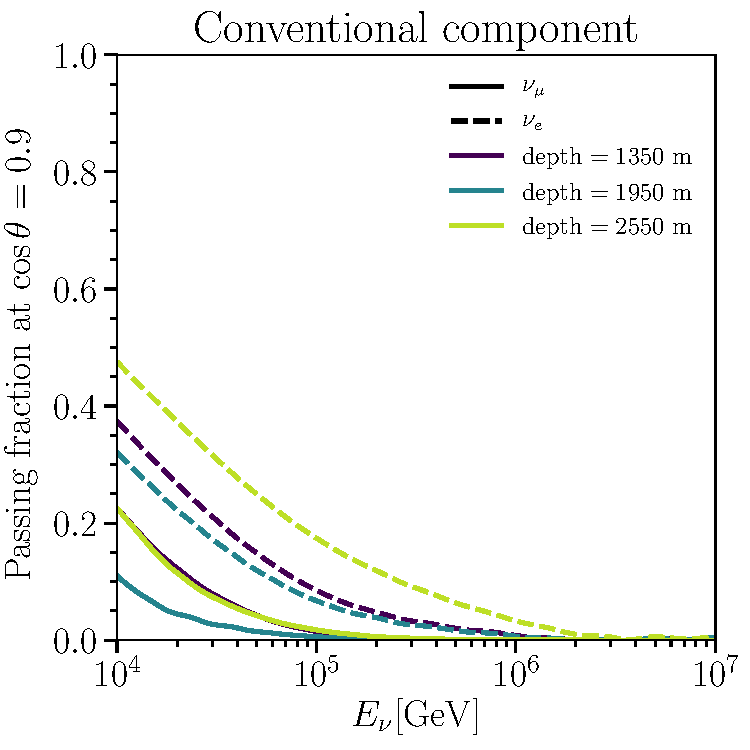
\includegraphics[width=0.3\linewidth]{results/HESE_Final_Paper/figures/conv_0_9_passing_fraction}} \\
	\subfloat{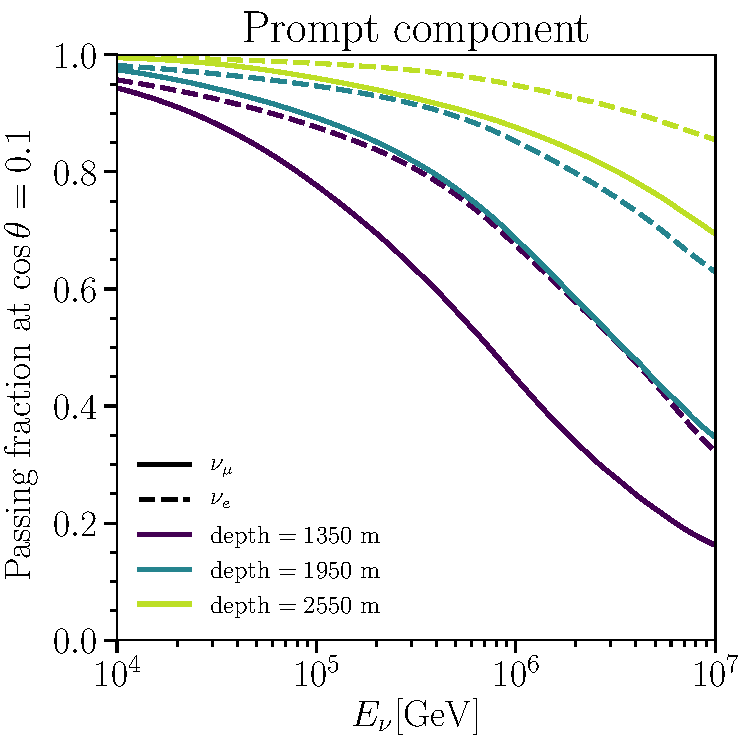
\includegraphics[width=0.3\linewidth]{results/HESE_Final_Paper/figures/prompt_0_1_passing_fraction}}
	\subfloat{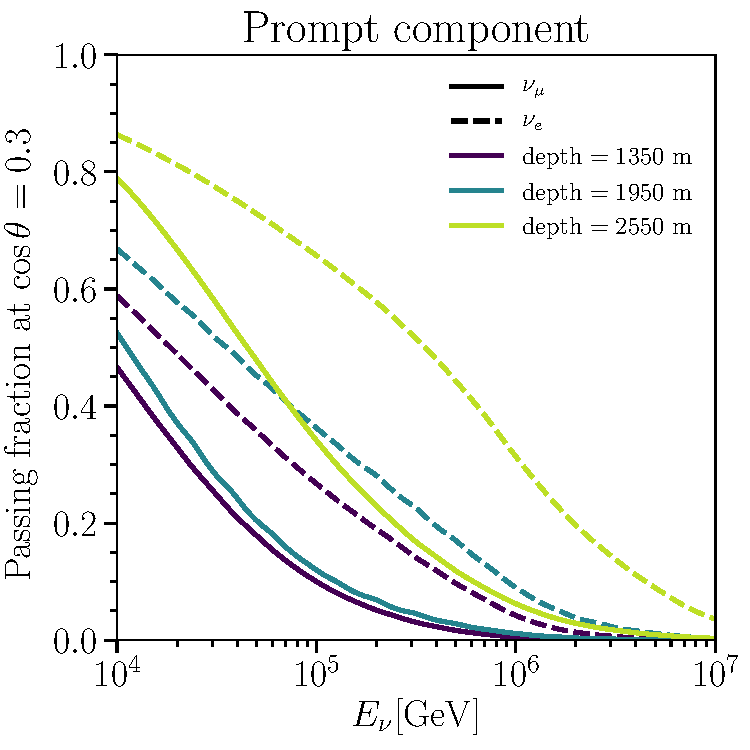
\includegraphics[width=0.3\linewidth]{results/HESE_Final_Paper/figures/prompt_0_3_passing_fraction}}
	\subfloat{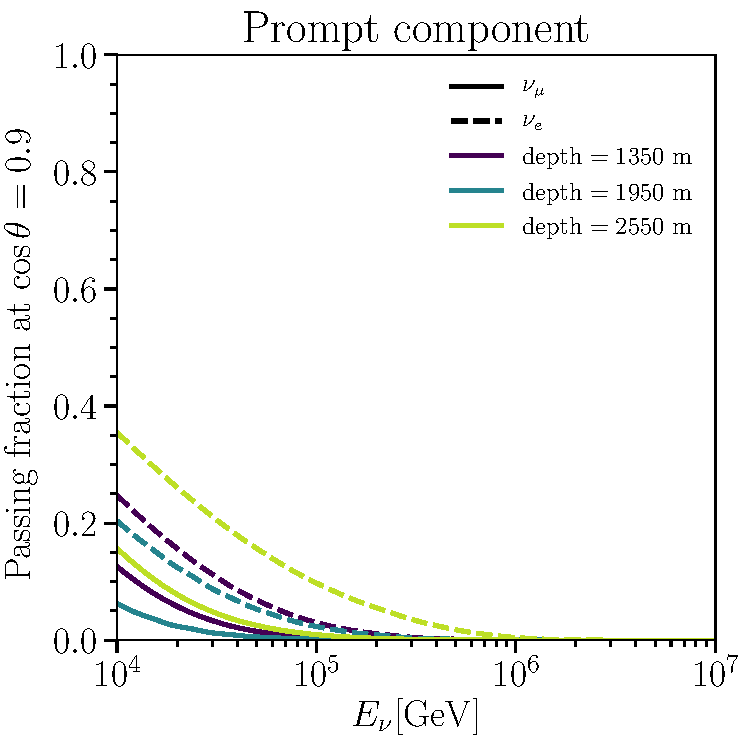
\includegraphics[width=0.3\linewidth]{results/HESE_Final_Paper/figures/prompt_0_9_passing_fraction}}
	\internallinenumbers
	\caption{\textbf{\textit{Conventional and prompt atmospheric component passing fraction.}}
		The top row of plots shows the atmospheric neutrino passing fraction as a function of the neutrino energy for a flux of neutrinos originating from pions and kaons, assuming the Hillas-Gaisser H3a~\cite{Gaisser:2013bla,Gaisser:2011cc,Hillas:2006ms} cosmic-ray model and SIBYLL 2.3c~\cite{Riehn:2017mfm} hadronic interaction model.
		While the bottom row of plots shows the atmospheric neutrino passing fraction for a flux of neutrinos originating from charmed hadrons under the same assumptions.
		Solid lines correspond to muon neutrinos and dashed lines to electron neutrinos.
		The different colors, from darkest to lightest, are for three different detector depths: 1350, 1950, and 2550 meters below the surface.
		The left, center, and right panel correspond to cosine of the zenith angles 0.1, 0.3, and 0.9 respectively (or zenith angles of $\SI{84.3}\degree$, $\SI{72.5}\degree$, and $\SI{25.8}\degree$).}\label{fig:passingfraction}
\end{figure*}

\textbf{TODO: Move the neutrino rate and muon rate figures to the analysis section?}
\textbf{TODO: Make some plots of the real neutrino flux before/after the veto.}

\begin{figure}
	\centering
	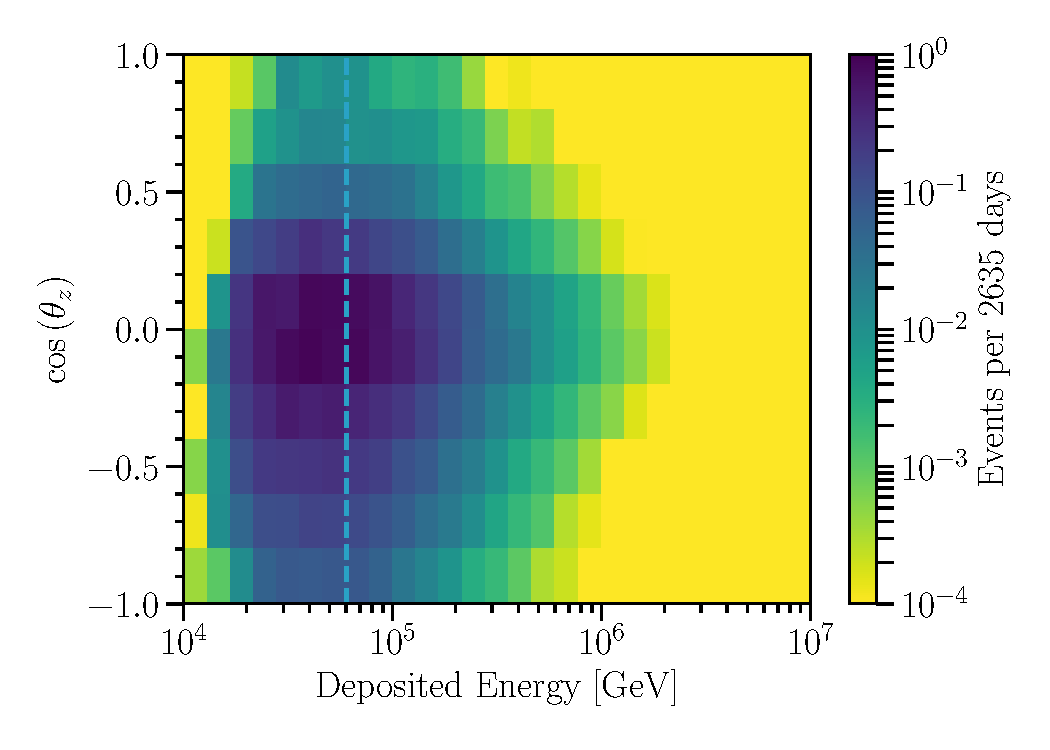
\includegraphics[width=\linewidth]{results/HESE_Final_Paper/figures/diffuse_hist_all_conv}
	\internallinenumbers
	\caption{\textbf{\textit{Expected distribution of atmospheric neutrinos produced by pions and kaons in the sample.}} Distribution of neutrinos that pass the veto as a function of the deposited energy and the cosine of the zenith angle assuming nominal values for the nuisance parameters.
		The dashed line at $\SI{60}\TeV$ marks the low energy cut of the analysis.
		Suppression in the down-going region is due to the veto, while suppression in the up-going region is due to absorption of neutrinos in the Earth.}\label{fig:conventional_distribution}
\end{figure}

\begin{figure}
	\centering
	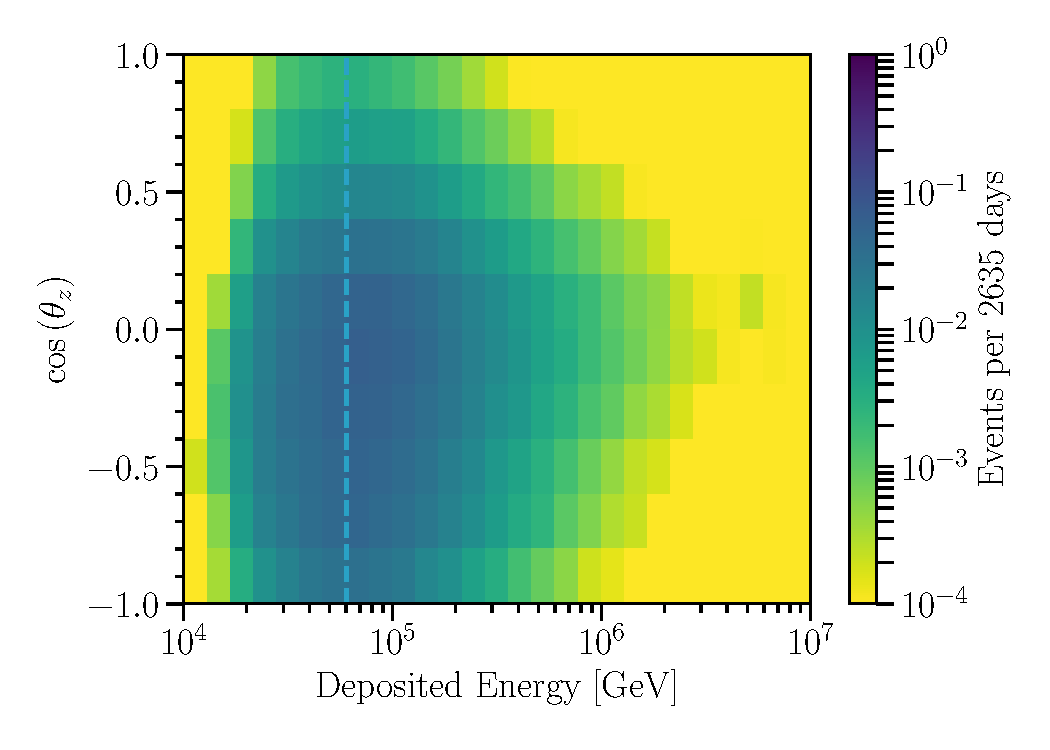
\includegraphics[width=\linewidth]{results/HESE_Final_Paper/figures/diffuse_hist_all_prompt}
	\internallinenumbers
	\caption{\textbf{\textit{Expected distribution of atmospheric neutrinos produced by charmed hadrons in the sample.}} Distribution of neutrinos that pass the veto as a function of the deposited energy and the cosine of the zenith angle assuming nominal nuisance parameters and the BERSS flux calculation for neutrinos from  charmed hadrons~\cite{Bhattacharya:2015jpa}.
		The dashed line at $\SI{60}\TeV$ marks the low energy cut of the analysis.
		Suppression in the down-going region is due to the veto, while suppression in the up-going region is due to absorption of neutrinos in the Earth.}\label{fig:prompt_distribution}
\end{figure}

\begin{figure}
	\centering
	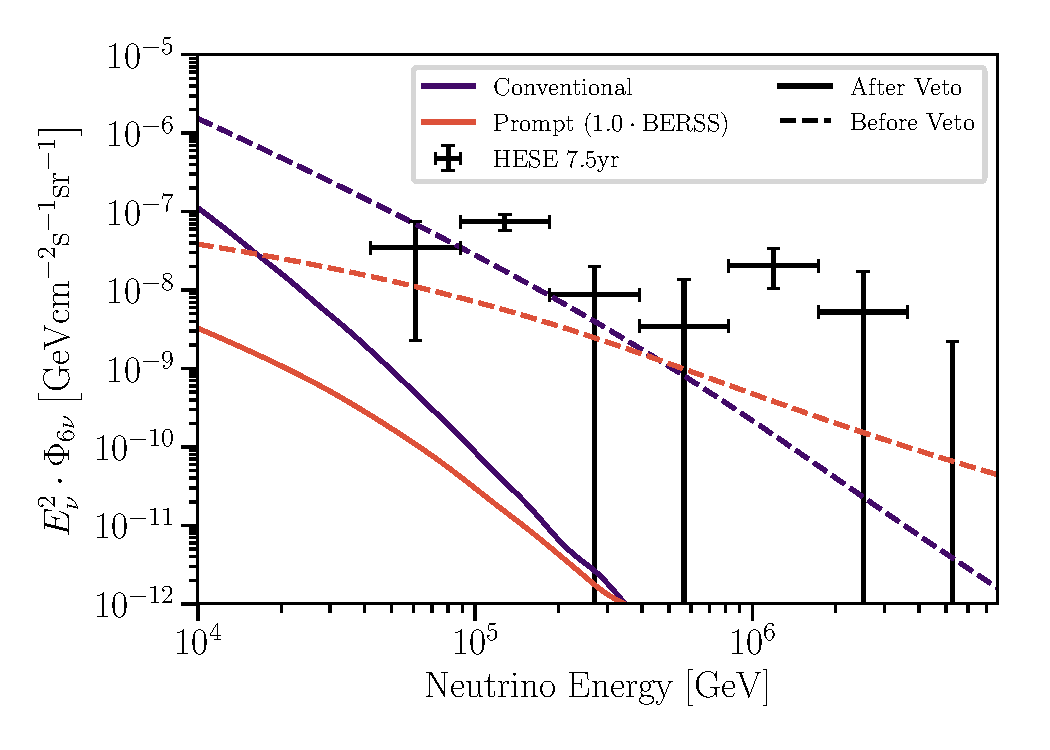
\includegraphics[width=\linewidth]{results/HESE_Final_Paper/figures/neutrino_spectrum}
	\internallinenumbers
	\caption{\textbf{\textit{All-sky astrophysical neutrino flux compared to down-going atmospheric neutrino fluxes before and after the veto.}}
		The atmospheric neutrino fluxes considered in this analysis are shown as dashed lines.
		The solid lines show the product of the atmospheric flux with the passing fraction averaged over depth at a zenith angle of $\SI{0}\degree$.
		The frequentist segmented power-law fit of the all-sky astrophysical flux assuming isotropy as described in \refsec{sec:generic_models} is shown in black.
		This comparison demonstrates the effect of the veto in the down-going region, where it is strongest.
		The suppression of the atmospheric flux becomes weaker towards the horizon, and is not present in the up-going region.
		The dashed lines labelled ``before-veto'' are equivalent to the up-going atmospheric fluxes, with or without the veto, neglecting Earth absorption effects.}
	\label{fig:neutrino_spectrum}
\end{figure}

\subsection{Muon background estimation}\label{sec:muon_background}
Finally, there is also the possibility of single muons that trigger the event selection without a neutrino interaction in the detector and still pass the veto.
The shape of the atmospheric muon and neutrino fluxes are closely related to each other, and bounded by the cosmic-ray flux so that they must be steeply falling.
The interaction of muons in the atmosphere and ice further softens the muon spectrum from that of cosmic rays.
Although there is uncertainty in the shape of the muon spectrum, the yield of muons from cosmic-ray air showers has more significant modelling uncertainties that stem from uncertainties in the hadronic interaction cross sections~\cite{Pierog:2017nes} and the cosmic-ray composition~\cite{Bluemer:2009zf}.
As we lack the capability to parameterize both the uncertainty in shape and normalization from first principles, we turn to data-driven techniques to constrain the size of this background.
Unfortunately, the data-driven techniques available do not provide us with enough events to determine the shape of the muon background.
For this reason we take a pragmatic approach to treat the muon component.
We use a simulation estimate of the muon flux shape which provides a reasonable estimate for a steeply falling muon spectrum, but neglects shape uncertainties.
The normalization is then constrained using a procedure that tags background muons in data.
The spectrum of atmospheric muons from cosmic-ray air showers is modelled by a parameterization of muons from air showers simulated with the \CORSIKA~\cite{Heck:1998vt} package assuming the Hillas-Gaisser H4a~\cite{Gaisser:2013bla} cosmic-ray flux model and SIBYLL 2.1~\cite{Ahn:2009wx} hadronic model.
A dedicated single muon simulation, called \MUONGUN~\cite{jvsthesis}, is weighted to this flux. 
%Due to the uncertainties in the muon yield of cosmic-ray air showers we use a data-based prior to constrain its normalization and only use the shape from simulation.
To construct the data based prior, a second veto layer inside the original outer veto layer is introduced.
Events that trigger the outer veto layer, but do not trigger this second inner veto layer, are tagged as muons that pass the inner veto.
The muon normalization from simulation is re-scaled from $N_\MUONGUN$ to $2.1\cdot N^\mu_\textmd{tagged}$ to match the number of tagged muons while accounting for the relative size of the fiducial volumes.
Thus, the baseline expected muon flux is given by
\begin{linenomath*}
	\begin{equation}
	\begin{split}
	\frac{d^3\Phi}{d E_\mu d \theta_{z,\mu} d d_\mu} ={}& \frac{d^3\Phi_\texttt{GaisserH4a}}{d E_\mu d \theta_{z,\mu} d d_\mu}(E_\mu, \theta_{z,\mu},d_\mu)\\* & \cdot \frac{2.1 \cdot N^\mu_\textmd{tagged}}{N_\MUONGUN},
	\end{split}
	\label{eq:muon_scaling}
	\end{equation}
\end{linenomath*}
where $\Phi_\texttt{GaisserH4a}$ is the aforementioned parameterization; and $E_\mu$, $\theta_{z,\mu}$, and $d_\mu$ are the muon energy, zenith, and depth at injection respectively.
In \reftab{tbl:tag_muons} we list the number of tagged muons observed per year; in total 17 muons were observed.
The expected distribution of passing atmospheric muon events is shown in \reffig{fig:muons} as a function of the deposited energy and reconstructed cosine of the zenith angle.
The prior on the atmospheric muon rate is chosen to be Gaussian with a $\SI{50}\percent$ standard deviation, this encompasses the statistical uncertainty of our muon background measurement.

\begin{figure}
	\centering
	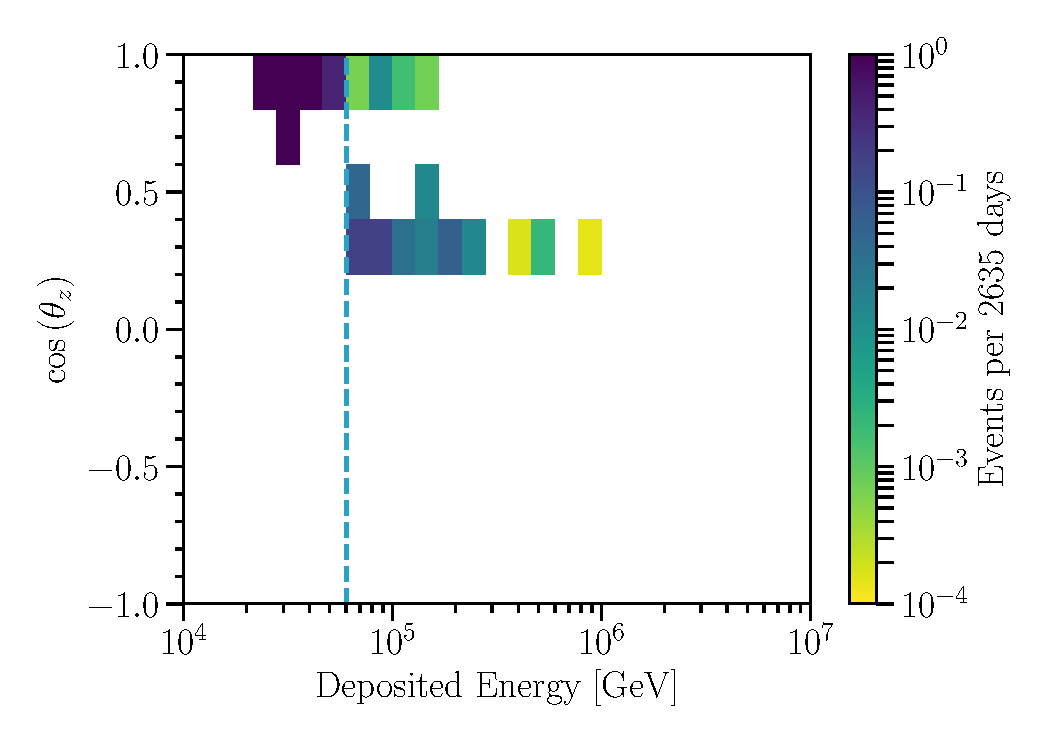
\includegraphics[width=\linewidth]{results/HESE_Final_Paper/figures/diffuse_hist_all_muons}
	\internallinenumbers
	\caption{\textbf{\textit{Expected distribution of atmospheric muons in the sample.}} Distribution of muons that pass the veto as calculated with \MUONGUN~as a function of the deposited energy and the cosine of the zenith angle.
		The normalization is set to match the data driven sub-detector study.
		The dashed line at $\SI{60}\TeV$ marks the low energy cut of the analysis.}\label{fig:muons}
\end{figure}

\begin{table}
	\centering
	% year & number of tagged muons
	\begin{tabular}{l r}
		\toprule
		Season & $N^\mu_{tagged}$ \\
		\midrule
		2010 & 2 \\
		2011 & 1 \\
		2012 & 1 \\
		2013 & 1 \\
		2014 & 2 \\
		2015 & 6 \\
		2016 & 2 \\
		2017 & 2 \\
		\midrule
		Total & 17 \\
		\bottomrule
	\end{tabular}
	\internallinenumbers
	\caption{\textbf{\textit{Number of tagged muons per season.}}
		Table shows the number of tagged muons used to construct the muon normalization prior.
		The first season, 2010, used a partial IceCube configuration with 79 strings, the rest of the seasons took data with the full configuration of 86 strings.
		The larger number of tagged muons in the 2015 season is believed to be a statistical fluctuation.
		The last season, 2017, represents only a partial year of data taking in this paper as the 2017 data processing was not yet completed at the time of this analysis.}\label{tbl:tag_muons}
\end{table}
